\chapter{Data sets and data generation}
\label{sec:data}

This chapter introduces the data used by \ldbcsnb. This includes the different
data types, the data schema, how it is generated and the different scale
factors.

\textbf{Warning.} This chapter describes the latest variant of the data set.
If you are looking for information on the Interactive workload, please also check 
\autoref{sec:legacy-data-sets}.

\section{Data Types}
\autoref{table:types} describes the different data types used in the benchmark.

\begin{table}[h]
    \centering
    \begin{tabular}{|>{\typeCell}p{\attributeColumnWidth}|p{\largeDescriptionColumnWidth}|}
        \hline
        \tableHeaderFirst{Type} & \tableHeader{Description} \\
        \hline
        ID &  integer type with 64-bit precision. All IDs within a single entity type (\eg Person, Message) are unique, but different entity types (\eg a Forum and a Tag) might have the same ID.\\
        \hline
        32-bit Integer &  integer type with 32-bit precision\\
        \hline
        64-bit Integer &  integer type with 64-bit precision\\
        \hline
        32-bit Float &  integer type with 32-bit precision\\
        \hline
        64-bit Float &  integer type with 64-bit precision\\
        \hline
        String & variable length text of size 80 Unicode characters\\
        \hline
        Long String & variable length text of size 256 Unicode characters\\
        \hline
        Text &  variable length text of size 2000 Unicode characters\\
        \hline
        Date &  date with a precision of a day, encoded as a string with the following format: \texttt{yyyy-mm-dd}, where \texttt{yyyy} is a four-digit integer representing the year,
        the year, \texttt{mm} is a two-digit integer representing the month and \texttt{dd} is a two-digit integer representing the day. \\
        \hline
        DateTime &  date with a precision of milliseconds, encoded as a string with the following format: \texttt{yyyy-mm-ddTHH:MM:ss.sss+00:00}, where \texttt{yyyy} is a four-digit integer representing the year,
        the year, \texttt{mm} is a two-digit integer representing the month and \texttt{dd} is a two-digit integer representing the day, \texttt{HH} is a two-digit integer representing the hour, \texttt{MM} is a two
        digit integer representing the minute and \texttt{ss.sss} is a five digit fixed point real number representing the seconds up to millisecond precision. Finally, the \texttt{+00:00} of the end represents the
        timezone, which should always be GMT (both for inputs and outputs).\\
        \hline
        Boolean &  logical type, taking the value of either \texttt{True} of \texttt{False}\\
        \hline
    \end{tabular}
    \caption{Description of the data types. Some types such as 32-bit  Float and 64-bit Integer are currently not used in the benchmark.}
    \label{table:types}
\end{table}


\section{Data Schema}

\autoref{fig:schema} shows the data schema in UML. The schema defines the
structure of the data used in the benchmark in terms of entities and their
relations. Data represents a snapshot of the activity of a social network
during a period of time. Data includes entities such as Persons, Organisations,
and Places. The schema also models the way persons interact, by means of the
friendship relations established with other persons, and the sharing of content
such as Messages (both textual and images), replies to Messages and likes to
Messages.  People form groups to talk about specific topics, which are
represented as Tags\footnote{Tags are basically equivalent to \emph{hashtags}
on contemporary social media sites. In this document, we occasionally use the term
\emph{topic} to refer to tags}. An example graph conforming the SNB schema is shown in \autoref{sec:example-graph}.

\ldbcsnb has been designed to be flexible and to target systems of different
nature and characteristics. As such, it does not force any particular internal
representation of the schema. The \datagen component
% described in \autoref{sec:data_generation}
supports multiple output data formats to
fit the needs of different types of systems, including RDF, relational DBMS and
graph DBMS.

\begin{figure}[htbp]
    \centering
    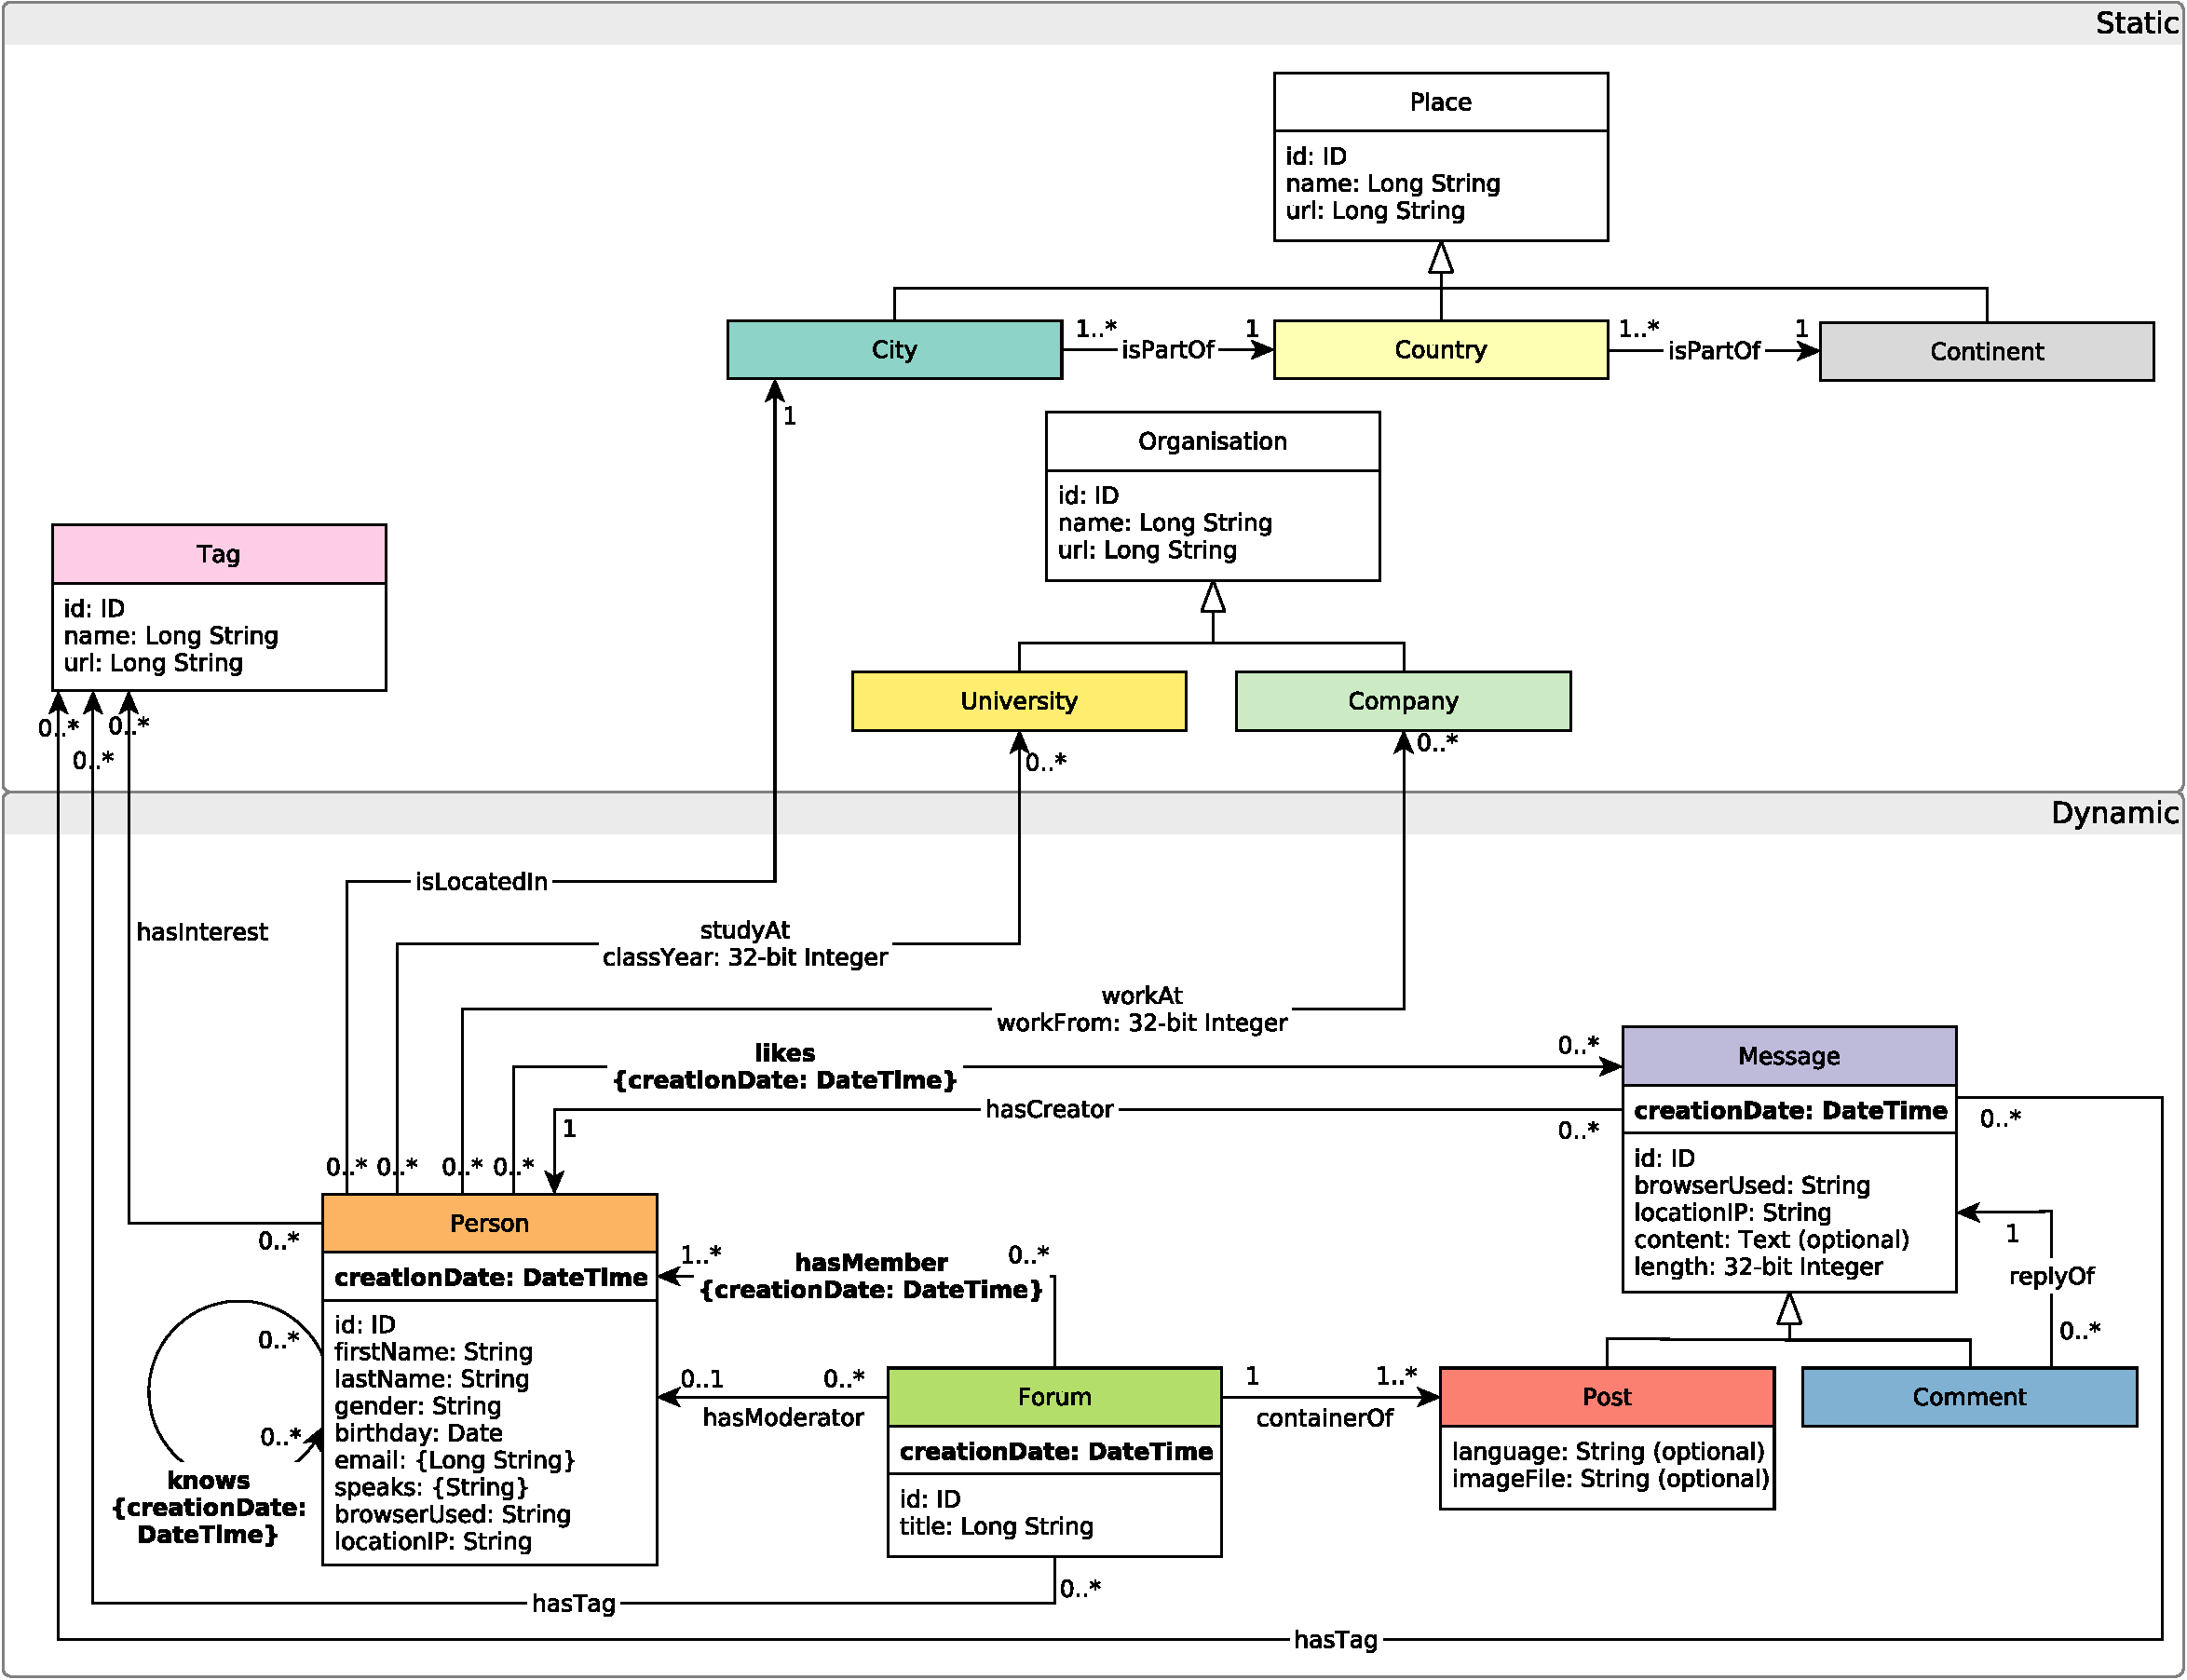
\includegraphics[scale=\yedscale]{figures/schema-comfortable}
    \caption{UML class diagram-style depiction of the \ldbcsnb graph schema. Note that the \textsf{knows} edges should be treated as undirected (but are serialized only in a single direction). The cardinality of the \textsf{hasModerator} edge has changed between version 0.3.x (where it was exactly 1) and version 0.4.x (where it is 0..1).}
    \label{fig:schema}
\end{figure}

The schema specifies different entities, their attributes and their relations.
All of them are described in the following sections.

\subsubsection*{Textual Restrictions and Notes}
\begin{itemize}
    \item Messageas always have a non-empty \texttt{content} attribute.
    \item Posts have either a \texttt{content} or an \texttt{imageFile} attribute (\ie they always have exactly one of them.) The one they do not have is represented with an empty string or with \texttt{NULL}.
    \item Posts in a forum can be created by a non-member person if and only if that person is the moderator of the Forum.
\end{itemize}

\subsection{Entities (Nodes)}

{\flushleft \textbf{City:}} a sub-class of a Place, and represents a
city of the real world. City entities are used to specify where persons live,
as well as where universities operate.

{\flushleft \textbf{Comment:}} a sub-class of a Message, and represents a
comment made by a person to an existing message (either a Post or a Comment).

{\flushleft \textbf{Company:}} a sub-class of an Organisation, and represents a company where persons work.

{\flushleft \textbf{Continent:}} a sub-class of a Place, and represents a continent of the real world.

{\flushleft \textbf{Country:}} a sub-class of a Place, and represents a country of the real world.
Countries are selected as the place of operation for Companies as well as the location of Messages.

{\flushleft \textbf{Forum:}} a meeting point where people
post messages. Forums are characterized by the topics (represented as tags)
people in the forum are talking about. Although from the schema's perspective
it is not evident, there exist three different types of
forums.  They are distinguished by their titles:

\begin{itemize}
    \item personal walls: ``Wall of \ldots''
    \item image albums: ``Album $k$ of \ldots''
    \item groups: ``Group for \ldots''
\end{itemize}

\autoref{table:forum} shows the attributes of the Forum entity.

\begin{table}[H]
    \begin{tabular}{|>{\varNameCell}p{\attributeColumnWidth}|>{\typeCell}p{\typeColumnWidth}|p{\descriptionColumnWidth}|}
        \hline
        \tableHeaderFirst{Attribute} & \tableHeader{Type} & \tableHeader{Description} \\
        \hline
        id & ID  & The identifier of the forum.\\
        \hline
        title & Long String  & The title of the forum.\\
        \hline
        creationDate & DateTime  & The date the forum was created.\\
        \hline
    \end{tabular}
    \caption{Attributes of the Forum entity.}
    \label{table:forum}
\end{table}


{\flushleft \textbf{Message:}} an abstract entity that represents a message
created by a person. \autoref{table:message} shows the attributes of the Message
abstract entity.

\begin{table}[H]
    \begin{tabular}{|>{\varNameCell}p{\attributeColumnWidth}|>{\typeCell}p{\typeColumnWidth}|p{\descriptionColumnWidth}|}
        \hline
        \tableHeaderFirst{Attribute} & \tableHeader{Type} & \tableHeader{Description} \\
        \hline
        id & ID  & The identifier of the message.\\
        \hline
        browserUsed & String  & The browser used by the Person to create the message.\\
        \hline
        creationDate & DateTime  & The date the message was created.\\
        \hline
        locationIP & String  & The IP of the location from which the message was created.\\
        \hline
        content & Text (optional)  & The content of the message.\\
        \hline
        length & 32-bit Integer  & The length of the content.\\
        \hline
    \end{tabular}
    \caption{Attributes of the Message interface.}
    \label{table:message}
\end{table}


{\flushleft \textbf{Organisation:}} an institution of the real
world. \autoref{table:organisation} shows the attributes of the Organisation
entity.

\begin{table}[H]
    \begin{tabular}{|>{\varNameCell}p{\attributeColumnWidth}|>{\typeCell}p{\typeColumnWidth}|p{\descriptionColumnWidth}|}
        \hline
        \tableHeaderFirst{Attribute} & \tableHeader{Type} & \tableHeader{Description} \\
        \hline
        id & ID  & The identifier of the organisation.\\
        \hline
        name & Long String  & The name of the organisation.\\
        \hline
        url & Long String  & The URL of the organisation.\\
        \hline
    \end{tabular}
    \caption{Attributes of the Organisation entity.}
    \label{table:organisation}
\end{table}


{\flushleft \textbf{Person:}} the avatar a real world person creates
when he/she joins the network, and contains various information about the
person as well as network related information. \autoref{table:person} shows
the attributes of the Person entity.

\begin{table}[H]
    \begin{tabular}{|>{\varNameCell}p{\attributeColumnWidth}|>{\typeCell}p{\typeColumnWidth}|p{\descriptionColumnWidth}|}
        \hline
        \tableHeaderFirst{Attribute} & \tableHeader{Type} & \tableHeader{Description} \\
        \hline
        id & ID  & The identifier of the person.\\
        \hline
        firstName & String  & The first name of the person.\\
        \hline
        lastName & String  & The last name of the person.\\
        \hline
        gender & String  & The gender of the person.\\
        \hline
        birthday & Date  & The birthday of the person.\\
        \hline
        email & \{Long String\}  & The set of emails the person has (cardinality: at least one).\\
        \hline
        speaks & \{String\}  & The set of languages the person speaks (cardinality: at least one).\\
        \hline
        browserUsed & String  & The browser used by the person when he/she registered to the social network.\\
        \hline
        locationIP & String  & The IP of the location from which the person was registered to the social network.\\
        \hline
        creationDate & DateTime  & The date the person joined the social network.\\
        \hline
    \end{tabular}
    \caption{Attributes of the Person entity.}
    \label{table:person}
\end{table}


{\flushleft \textbf{Place:}} a place in the world.
\autoref{table:place} shows the attributes of the Place entity. Note, each Place has additional parameters: longitude and latitude, which are not exposed. These are used internally for sorting places.

\begin{table}[H]
    \begin{tabular}{|>{\varNameCell}p{\attributeColumnWidth}|>{\typeCell}p{\typeColumnWidth}|p{\descriptionColumnWidth}|}
        \hline
        \tableHeaderFirst{Attribute} & \tableHeader{Type} & \tableHeader{Description} \\
        \hline
        id & ID  & The identifier of the place.\\
        \hline
        name & Long String  & The name of the place.\\
        \hline
        url & Long String  & The URL of the place.\\
        \hline
    \end{tabular}
    \caption{Attributes of the Place entity.}
    \label{table:place}
\end{table}


{\flushleft \textbf{Post:}} a sub-class of Message, that is posted in a
forum. Posts are created by persons into the forums where they belong.
Posts contain either content or imageFile, always one of them but never both.
The one they do not have is an empty string.
\autoref{table:post} shows the attributes of the Post entity.

\begin{table}[H]
    \begin{tabular}{|>{\varNameCell}p{\attributeColumnWidth}|>{\typeCell}p{\typeColumnWidth}|p{\descriptionColumnWidth}|}
        \hline
        \tableHeaderFirst{Attribute} & \tableHeader{Type} & \tableHeader{Description} \\
        \hline
        language & String (optional) & The language of the post. Mutually exclusive with \texttt{imageFile}. \\
        \hline
        imageFile & String (optional) & The image file of the post. Mutually exclusive with \texttt{language}.\\
        \hline
    \end{tabular}
    \caption{Attributes of the Post entity.}
    \label{table:post}
\end{table}


{\flushleft \textbf{Tag:}} a topic or a concept. Tags are used to
specify the topics of forums and posts, as well as the topics a person is
interested in. \autoref{table:tag} shows the atltributes of the Tag entity.

\begin{table}[H]
    \begin{tabular}{|>{\varNameCell}p{\attributeColumnWidth}|>{\typeCell}p{\typeColumnWidth}|p{\descriptionColumnWidth}|}
        \hline
        \tableHeaderFirst{Attribute} & \tableHeader{Type} & \tableHeader{Description} \\
        \hline
        id & ID  & The identifier of the tag.\\
        \hline
        name & Long String  &  The name of the tag.\\
        \hline
        url & Long String  &  The URL of the tag.\\
        \hline
    \end{tabular}
    \caption{Attributes of the Tag entity.}
    \label{table:tag}
\end{table}


{\flushleft \textbf{TagClass:}} a class used to build a hierarchy of tags. \autoref{table:tagclass} shows the attributes of the TagClass entity.

\begin{table}[H]
    \begin{tabular}{|>{\varNameCell}p{\attributeColumnWidth}|>{\typeCell}p{\typeColumnWidth}|p{\descriptionColumnWidth}|}
        \hline
        \tableHeaderFirst{Attribute} & \tableHeader{Type} & \tableHeader{Description} \\
        \hline
        id & ID  & The identifier of the tagclass.\\
        \hline
        name & Long String  &  The name of the tagclass.\\
        \hline
        url & Long String  &  The URL of the tagclass.\\
        \hline
    \end{tabular}
    \caption{Attributes of the TagClass entity.}
    \label{table:tagclass}
\end{table}


{\flushleft \textbf{University:}} a sub-class of Organisation,
and represents an institution where persons study.

\subsection{Relations (Edges)}

Relations (edges) connect entities of different types. The endpoint entities are defined by their ``id'' attribute.
Edge instances starting from or ending in a given node are treated as a set, \ie no ordering is defined on the edges.
Multiple edges (\ie edges of the same type between two entity instances) are not allowed in SNB graphs.

\begin{longtable}{|>{\varNameCell}p{2.5cm}|>{\typeCell}p{2.5cm}|>{\typeCell}p{2.5cm}|>{\edgeDirectionCell}c|p{6.5cm}|}
    \hline
     \tableHeaderFirst{Name} & \tableHeader{Tail} & \tableHeader{Head} & \tableHeader{Type} & \tableHeader{Description} \\
     \hline
     containerOf & Forum[1] & Post[1..*] & D & A Forum and a Post contained in it\\
     \hline
     hasCreator & Message[0..*] & Person[1] & D & A Message and its creator (Person)\\
     \hline
     hasInterest & Person[0..*] & Tag[0..*] & D & A Person and a Tag representing a topic the person is interested in\\
     \hline
     hasMember & Forum[0..*] &  Person[1..*] & D & A Forum and its member (Person)

     In version 0.3.x:

     \attributeTable{joinDate}{DateTime}{The Date the person joined the Forum}

     In version 0.4.0+:

     \attributeTable{creationDate}{DateTime}{The Date the person joined the Forum}

     \\
     \hline
     hasModerator & Forum[0..*] &
     \textrm{In version 0.3.x:}
     
     Person[1]
     
     \textrm{In version 0.4.0+:}

     Person[0..1]
     & D & A Forum and its moderator (Person) \\
     \hline
     hasTag & Message[0..*] & Tag[0..*] & D & A Message and a Tag representing the message's topic \\
     \hline
     hasTag & Forum[0..*] & Tag[0..*] & D & A Forum and a Tag representing the forum's topic \\
     \hline
     hasType & Tag[0..*] & TagClass[1] & D & A Tag and a TagClass the tag belongs to \\
     \hline
     isLocatedIn & Company[0..*] & Country[1] & D & A Company and its home Country \\
     \hline
     isLocatedIn & Message[0..*] & Country[1] & D & A Message and the Country from which it was issued \\
     \hline
     isLocatedIn & Person[0..*] & City[1] & D & A Person and their home City \\
     \hline
     isLocatedIn & University[0..*] & City[1] & D &  A University and the City where the university is \\
     \hline
     isPartOf & City[1..*] & Country[1] & D & A City and the Country it is part of \\
     \hline
     isPartOf & Country[1..*] & Continent[1] & D & A Country and the Continent it is part of \\
     \hline
     isSubclassOf & TagClass[0..*] & TagClass[0..1] & D & A TagClass and its parent TagClass \\
     \hline
     knows & Person[0..*] & Person[0..*] & U & Two Persons that know each other.
     Note that
     (1)~the knows edges are undirected (all other edge types are directed and
     (2)~to avoid duplications, these edges are only serialized to one direction and it is the responsibility of the loader/implementation component to treat them as undirected.

     \attributeTable{creationDate}{DateTime}{The date the knows relation was established}

     \\
     \hline
     likes & Person[0..*] & Message[0..*] & D & A Person that likes a Message

     \attributeTable{creationDate}{DateTime}{The date the like was issued}

     \\
     \hline
     replyOf & Comment[0..*] & Message[1] & D & A Comment and the Message it replies \\
     \hline
     studyAt & Person[0..*] & University[0..*] & D & A Person and a University it has studied

     \attributeTable{classYear}{32-bit Integer}{The year the person graduated}

     \\
     \hline
     workAt & Person[0..*] & Company[0..*] & D & A Person and a Company it works

     \attributeTable{workFrom}{32-bit Integer}{The year the person started to work at that Company}

     \\
     \hline
 \caption{Description of the data relations. Type -- \texttt{D}: directed edge, \texttt{U}: undirected edge.}
 \label{table:relations}
\end{longtable}


\subsection{Domain Concepts}

A \emph{thread} consists of Messages, starting with a single Post and the Comments that -- either directly or transitively -- reply to that Post.

\section{Data Generation}
\label{sec:data_generation}

\ldbcsnb provides \datagen (Data Generator), which produces synthetic
datasets following the schema described above. Data
produced mimics a social network's activity during a period of time. Three
parameters determine the generated data: the number of persons, the number of
years simulated, and the starting year of simulation. \datagen is defined by the
following characteristics:

\begin{itemize}
    \item \textbf{Realism.} Data generated by \datagen mimics the
        characteristics of those found in a real social network. In \datagen,
        output attributes, cardinalities, correlations and distributions have
        been finely tuned to reproduce a real social network in each of its
        aspects. On the one hand, it is aware of the  data and link distributions
        found in a real social network such as Facebook. On the other hand, it
        uses real data from DBpedia, such as property dictionaries, which are
        used to ensure that attribute values are realistic and correlated.
    \item \textbf{Scalability.} Since \ldbcsnb targets systems of different
        scales and budgets, \datagen is capable of generating datasets of
        different sizes, from a few Gigabytes to Terabytes. \datagen is
        implemented following the MapReduce parallel paradigm, allowing the
        generation of small datasets in single node machines, as well as large
        datasets on commodity clusters.
    \item \textbf{Determinism.} \datagen is deterministic regardless of the number
        of cores/machines used to produce the data. This important feature
        guarantees that all Test Sponsors will face the same dataset,
        thus, making the comparisons between different systems fair and the
        benchmarks' results reproducible.
    \item \textbf{Usability.} \ldbcsnb is designed to have an affordable entry
        point. As such, \datagen's design is  severely influenced by this
        philosophy, and therefore it is designed to be as easy to use as
        possible.
\end{itemize}


\subsection{Resource Files}

\datagen uses a set of resource files with data
extracted from DBpedia. Conceptually, \datagen generates attribute's
values following a property dictionary model that is defined by

\begin{itemize}
    \item a dictionary $D$
    \item a ranking function $R$
    \item a probability function $F$
\end{itemize}

Dictionary $D$ is a fixed set of values. The ranking function $R$ is a bijection
that assigns to each value in a dictionary a unique rank between 1 and $|D|$.
The probability density function $F$ specifies how the data generator chooses
values from dictionary $D$ using the rank for each term in the dictionary. The
idea to have a separate ranking and probability function is motivated by the
need of generating correlated values: in particular, the ranking function is
typically parameterized by some parameters: different parameter values result
in different rankings. For example, in the case of a dictionary of property
firstName, the popularity of first names might depend on the gender, country
and birthday properties. Thus, the fact that the popularity of first names in
different countries and times is different, is reflected by the different ranks
produced by function $R$ over the full dictionary of names.  \datagen uses a
dictionary for each literal property, as well as ranking functions for all
literal properties. These are materialized in a set of resource files, which
are described in \autoref{table:property_dictionaries}.

\begin{table}[H]
\begin{tabular}{|p{4cm}|p{12cm}|}
    \hline
    \tableHeaderFirst{Resource Name} & \tableHeader{Description} \\
    \hline
    Browsers & Contains a list of web browsers and their probability to be used. It is used to set the browsers used by the users.\\
    \hline
    Cities by Country & Contains a list of cites and the country they belong. It is used to assign cities to users and universities.\\
    \hline
    Companies by Country & Contains the set of companies per country. It is used to set the countries where companies operate.\\
    \hline
    Countries & Contains a list of countries and their populations. It is used to obtain the amount of people generated for each country.\\
    \hline
    Emails & Contains the set of email providers. It is used to generate the email accounts of persons.\\
    \hline
    IP Zones & Contains the set of IP ranges assigned to each country. It is used to assign the IP addresses to users.\\
    \hline
    Languages by Country & Contains the set of languages spoken in each country. It is used to set the languages spoken by each user.\\
    \hline
    Name by Country & Contains the set of names and the probability to appear in each country. It is used to assign names to persons, correlated with their countries.\\
    \hline
    Popular places by Country & Contains the set of popular places per country. These are used to set where images attached to posts are taken from.\\
    \hline
    Surnames' by Country & Contains the set of surnames and the probability to appear in each country. It is used to assign surnames to persons, correlated with their countries.\\
    \hline
    Tags by Country & Contains a set of tags and their probability to appear in each country. It is used to assign the interests to persons and forums.\\
    \hline
    Tag Classes & Contains, for each tag, the classes it belongs to.\\
    \hline
    Tag Hierarchies & Contains, for each tagClass, their parent tagClass.\\
    \hline
    Tag Matrix & Contains, for each tag, the correlation probability with the other tags. It is used enrich the tags associated to messages.\\
    \hline
    Tag Text & Contains, for each tag, a text. This is used to generate the text for messages.\\
    \hline
    Universities by City & Contains the set of universities per city. It is used to set the cities where universities operate.\\
    \hline
\end{tabular}
\caption{Resource files.}
\label{table:property_dictionaries}
\end{table}


\subsection{Graph Generation}

\autoref{fig:generation_process} conceptually depicts the full data
generation process. The first step loads all the dictionaries and resource
files, and initializes the \datagen parameters.  Second, it generates all the
Persons in the graph, and the minimum necessary information to operate. Part of
this information are the interests of the persons, and the number of knows
relationships of every person, which is guided by a degree distribution
function similar to that found in Facebook~\cite{facebook_anatomy}.

The next three steps are devoted to the creation of knows relationships.  An
important aspect of real social networks, is the fact that similar persons
(with similar interests and behaviors) tend to be connected. This is known as
the Homophily principle~\cite{mcpherson2001birds,DBLP:journals/socnet/BaroneC18}, and implies the presence of
a larger amount of triangles than that expected in a random network. In order
to reproduce this characteristic, \datagen generates the edges by means of
correlation dimensions.  Given a person, the probability to be connected to
another person is typically skewed with respect to some similarity between the
persons. That is, for a person $p$ and for a small set of persons that are
somehow similar to it, there is a high connectivity probability, whereas for
most other persons, this probability is quite low. This knowledge is
exploited by \datagen to reproduce correlations.

\begin{figure}[htb]
    \centering
    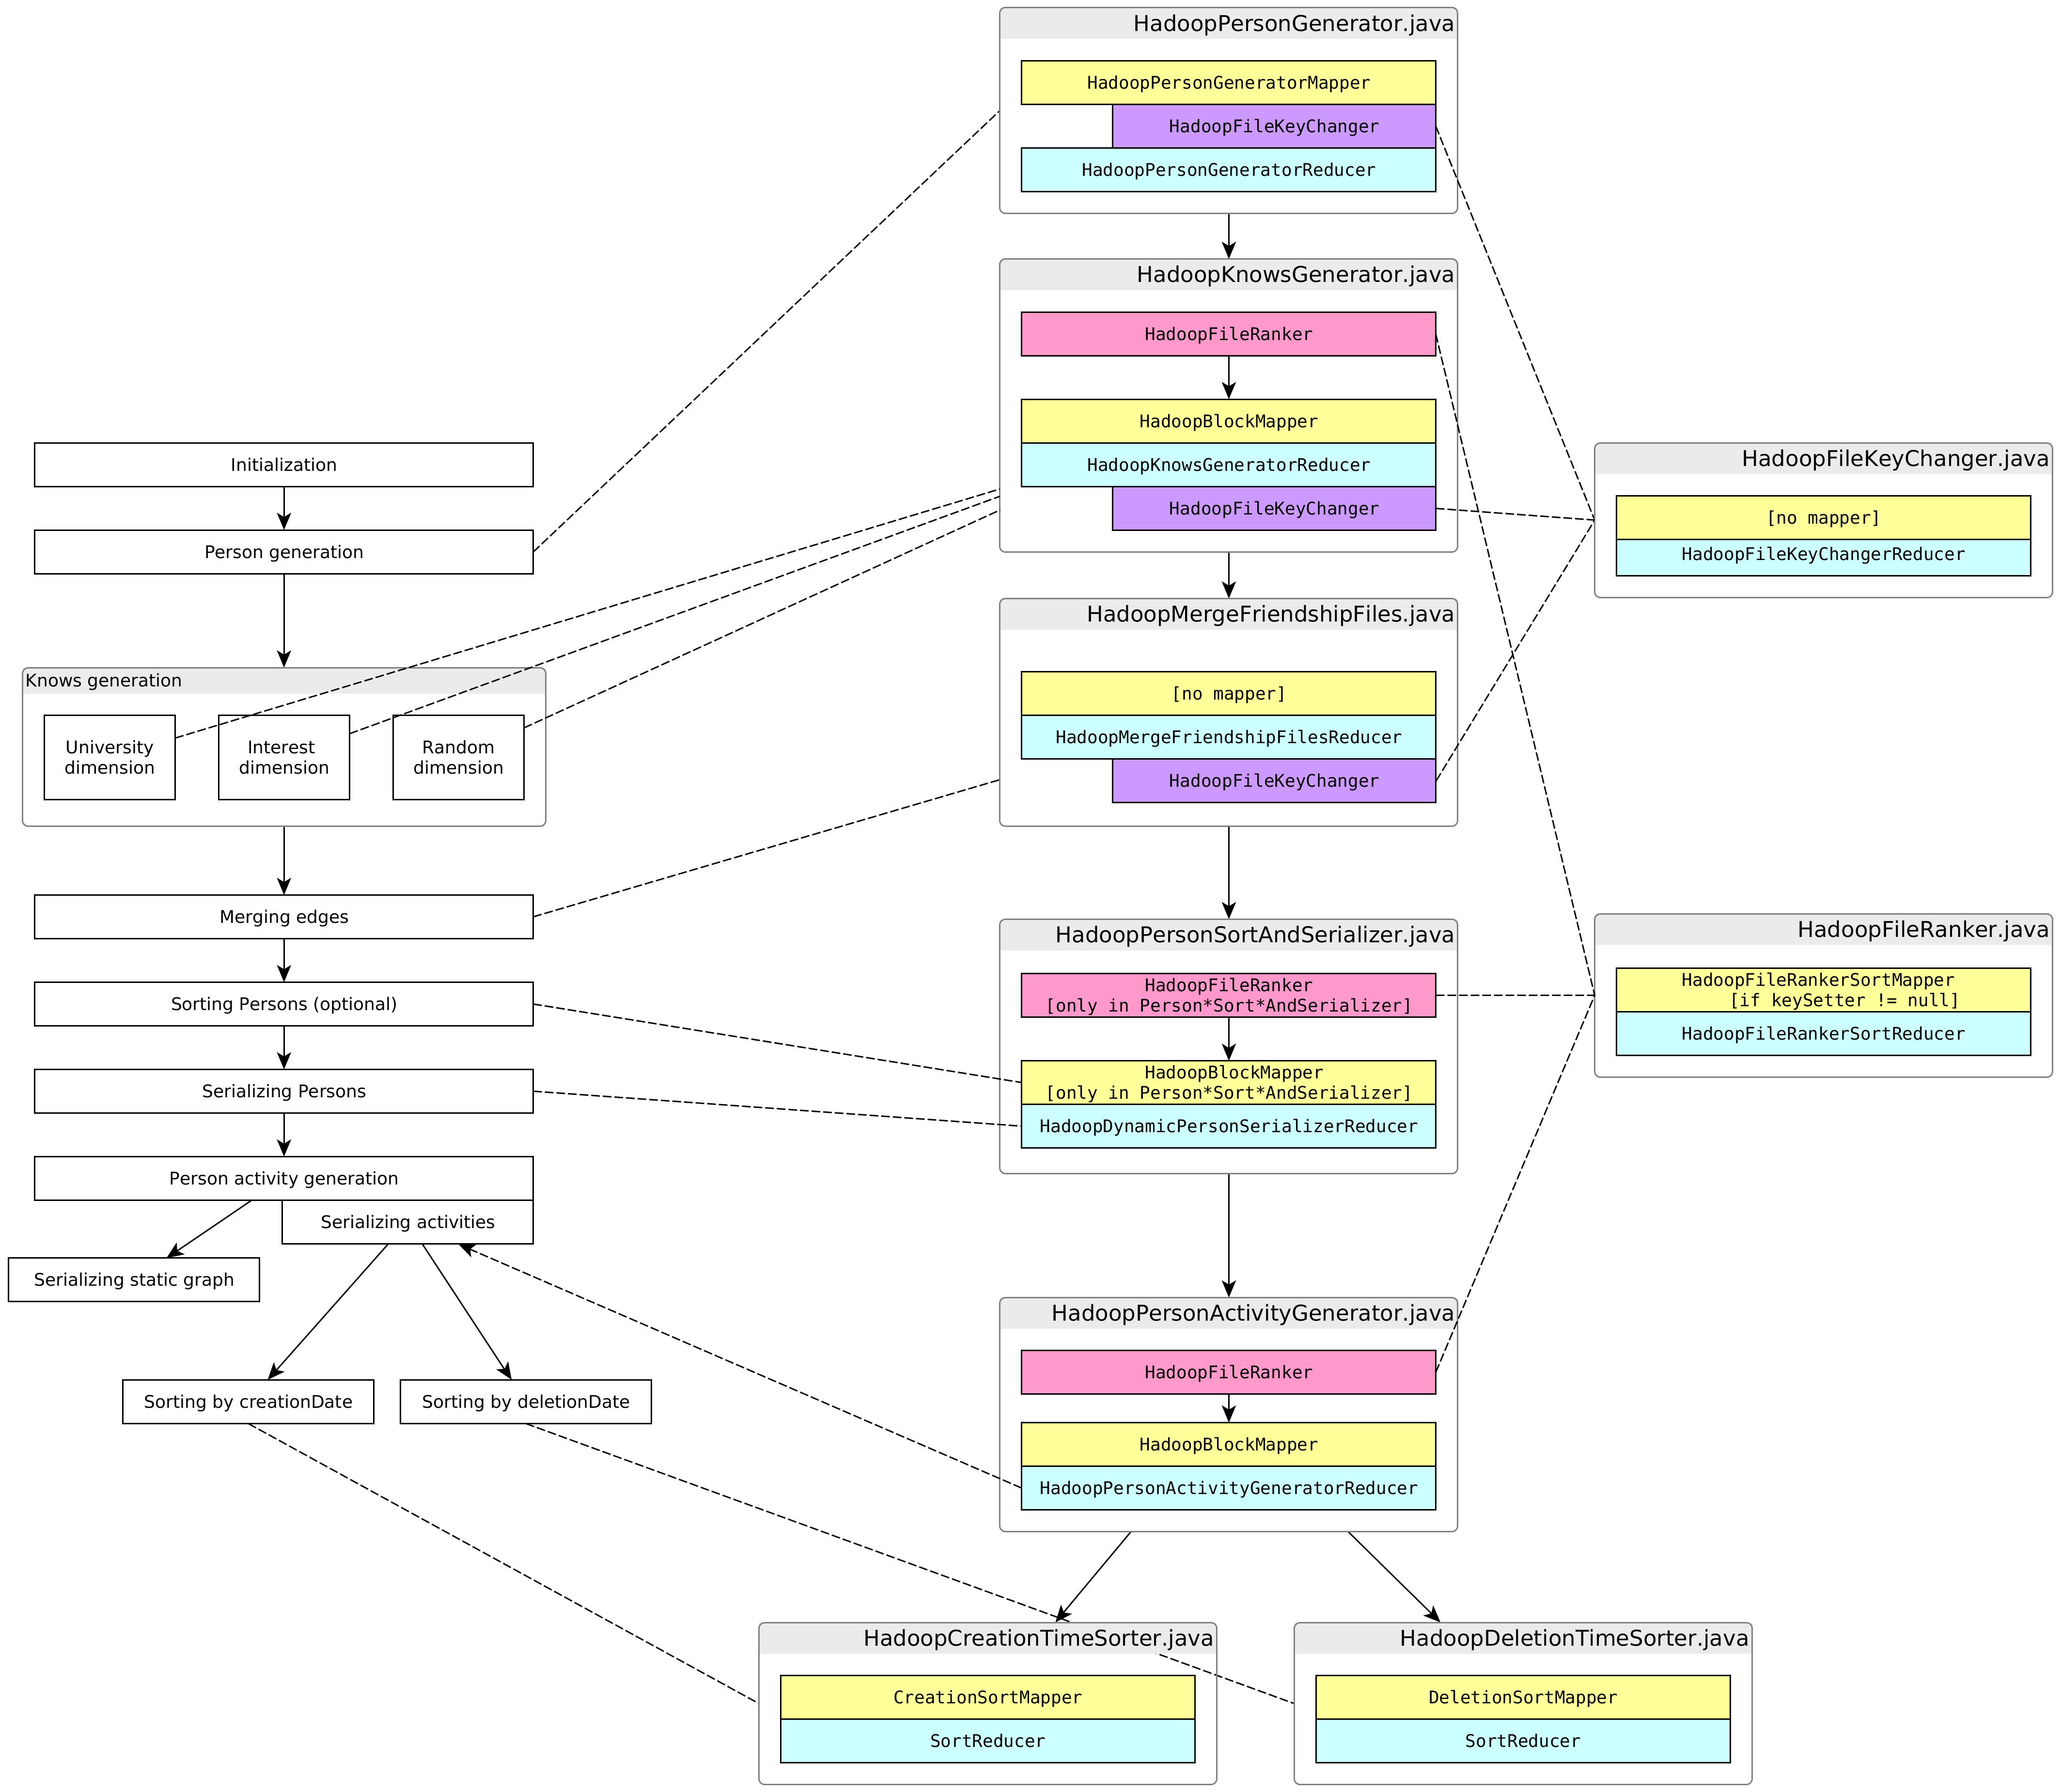
\includegraphics[scale=\yedscale]{figures/datagen-workflow}
    \caption{The \datagen generation process.}
    \label{fig:generation_process}
\end{figure}

Given a similarity function $M(p) : p \rightarrow [0, \infty)$ that gives a score to a person,
with the characteristic that two similar persons will have similar scores, we
can sort all the persons by function $M$ and compare a person $p$ against only the
$K$ neighbouring persons in the sorted array. The consequence of this approach is
that similar persons are grouped together, and the larger the
distance between two persons indicates a monotonic increase in their similarity
difference. In order to choose the persons to connect, \datagen uses a geometric
probability distribution that provides a probability for picking persons to
connect, that are between 1 and $K$ positions apart in the similarity
ranking.

Similarity functions and probability distribution functions over ranked
distance drive what kind of persons will be connected with an edge, not how
many. As stated above, the number of friends of a person is determined by a
Facebook-like distribution. The edges that will be connected to a person $p$,
are selected by randomly picking the required number of edges according to the
correlated probability distributions as discussed before. In the case that
multiple correlations exist, another probability function is used to divide the
intended number of edges between the various correlation dimensions. In \datagen,
three correlated dimensions are chosen: the first one depends on where the
person studied and when, and the second correlation dimension depends on the
interests of the person, and the third one is random (to reproduce the random
noise present in real data). Thus, \datagen has a Facebook-like distributed node
degree, and a predictable (but not fixed) average split between the reasons for
creating edges.

In the next step, a person's activity, in the form of forums, posts and comments
is created. \datagen reproduces the fact that people with a larger number of
friends have a higher activity, and hence post more photos and comments to a
larger number of posts. Another important characteristic of real persons'
activity in social network, are time correlations.  Usually, person' posts
creation in a social network is driven by real world events.  For
instance, one may think about an important event such as the elections in a
country, or a natural disaster. Around the time these events occur, network
activity about these events' topics sees an increase in volume. \datagen
reproduces these characteristics with the simulation of what we name as
flashmob events.  Several events are generated randomly at the beginning of the
generation process, which are assigned a random tag, and are given a time and
an intensity which represents the repercussion of the event in the real world.
When persons' posts are created, some of them are classified as flashmob posts,
and their topics and dates are assigned based on the generated flashmob events.
The volume of activity around this events is modeled following a model similar
to that described in~\cite{DBLP:conf/kdd/LeskovecBKT08}. Furthermore, in order to reproduce the
more uniform every day person activity, \datagen also generates posts uniformly
distributed along all the simulated time.

Finally, in the last step the data is serialized into the output files.

\subsection{Distributions, Parameters, and Quirks}
\label{sec:distr-param}

Interesting quirks:
\begin{itemize}
\item A Person is not a member of their Wall but they are its moderator, they do not have a hasMember edge.
\item Each Album generated for Person will have approximately 70\% of their friends as members.
\item A given Person has a 5\% chance of being a moderator of a set of groups.
\item Group membership is composed of 30\% from the moderator's friends and the remainder is chosen randomly (from the block the person is in).
\item Comments are only made in Walls and Groups.
\item Messages can only receive likes during a 7-day window after their creation.
\item Comments always occur within one day of Message they are replying to. The creation date is generated following the power-law distribution in Figure \ref{fig:comments_dist}. The mean delay between Comments and their parent Message is 6.85 hours.
\item Flashmob events span a 72-hour time window with a specific event time in the middle of the window; there are 36 hours each side of the specific event time. Following the distribution in Figure \ref{fig:flashmob_dist} posts are generated either side of flashmob event time, posts are clustered around the specific event time.
\end{itemize}

\begin{figure}[htb]
  \centering
  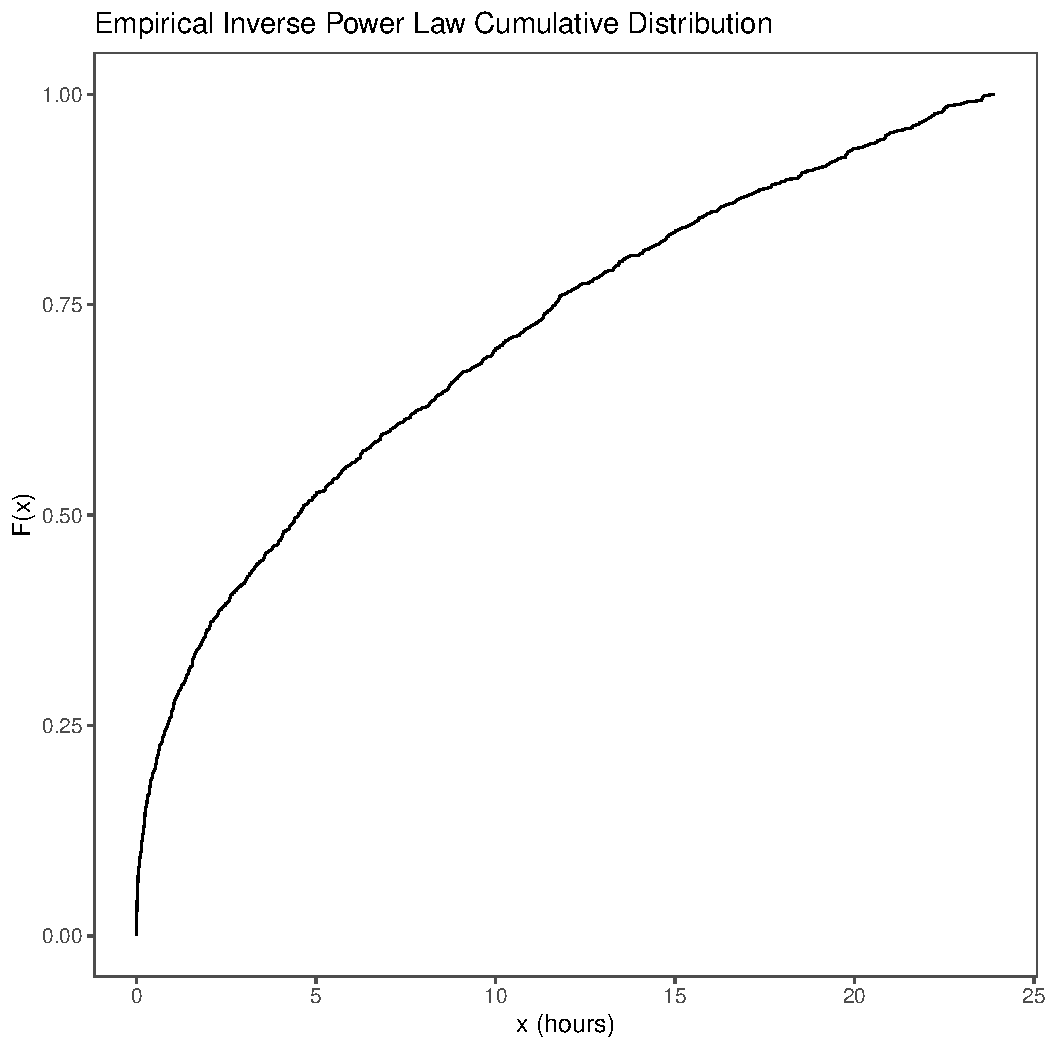
\includegraphics[scale=\yedscale]{figures/comments_power_law}
  \caption{The power-law used to generate comments.}
  \label{fig:comments_dist}
\end{figure}

\begin{figure}[htb]
  \centering
  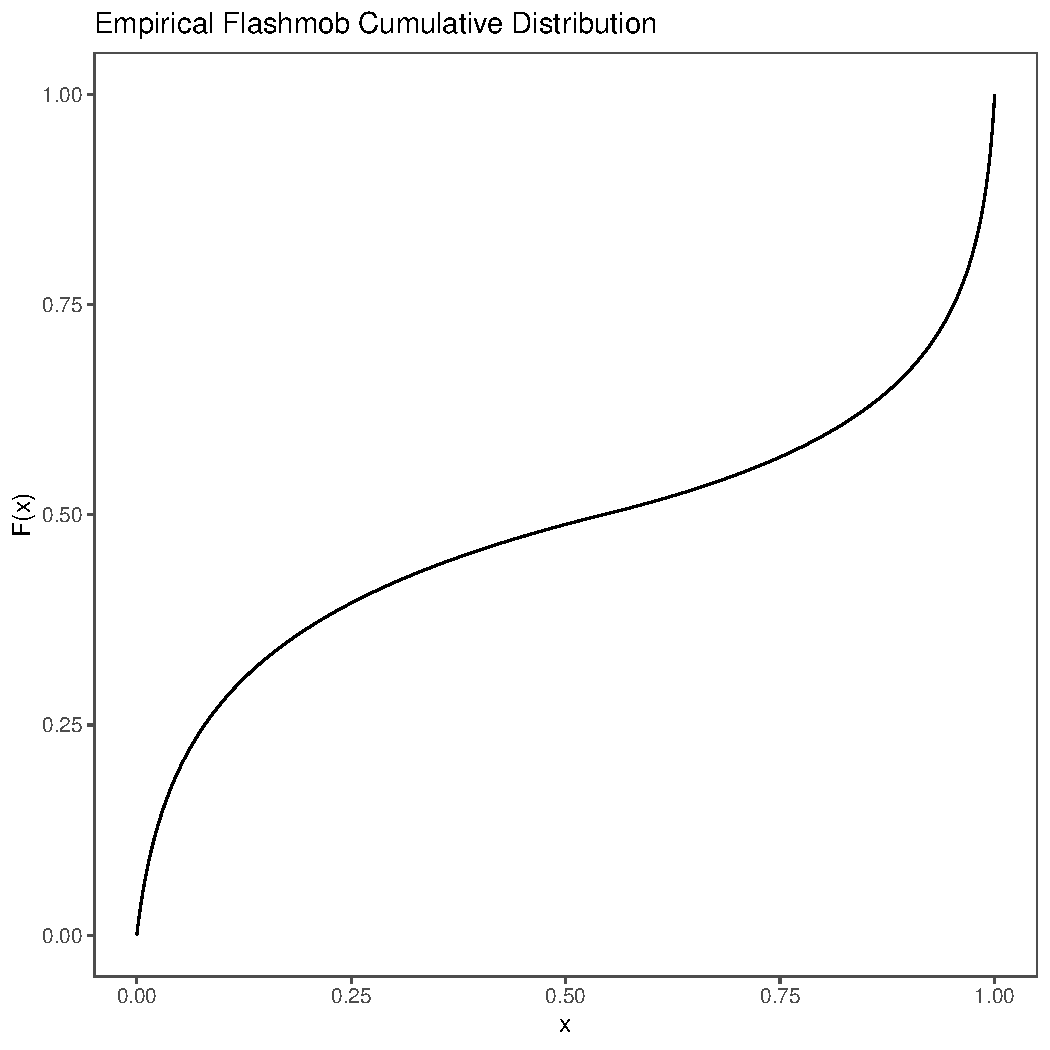
\includegraphics[scale=\yedscale]{figures/flashmob_dist}
  \caption{The distribution used to generate posts during flashmob events.}
  \label{fig:flashmob_dist}
\end{figure}

\subsection{Implementation Details}

\datagen is implemented using the MapReduce parallel paradigm. In MapReduce, a
Map function runs on different parts of the input data, in parallel and on many
node clusters. This function processes the input data and produces for each
result a key. Reduce functions then obtain this data and Reducers run in
parallel on many cluster nodes. The produced key simply determines the Reducer
to which the results are sent. The use of the MapReduce paradigm allows the
generator to scale considerably, allowing the generation of huge datasets by
using clusters of machines.

In the case of \datagen, the overall process is divided into three MapReduce jobs.
In the first job, each mapper generates a subset of the persons of the graph. A
key is assigned to each person using one of the similarity functions described
above. Then, reducers receive the key-value pairs sorted by the key,
generate the knows relations following the described windowing process, and
assign to each person a new key based on another similarity function, for the
next MapReduce pass.  This process can be successively repeated for additional
correlation dimension.  Finally, the last reducer generates the remaining
information such as forums, posts and comments.

\section{Output Data}

For each scale factor, \datagen produces three different artefacts:
\begin{itemize}
  \item \textbf{Dataset:} The dataset to be bulk loaded by the SUT. In the Interactive workload, it corresponds to roughly the 90\% of the total generated network.
  \item \textbf{Update Streams:} A set of update streams containing update
    queries, which are used by the driver to generate the update queries of the
    workloads. This update
    streams correspond to the remaining 10\% of the generated dataset.
  \item \textbf{Substitution Parameters:} A set of files containing the
    different parameter bindings that will be used by the driver to generate the
    read queries of the workloads.
\end{itemize}

\subsection{Scale Factors}
\label{sec:scale-factors}

\ldbcsnb defines a set of scale factors (SFs), targeting systems of different sizes and budgets.
SFs are computed based on the ASCII size \emph{in Gibibytes} of the generated output files using the \textsf{csv-singular-merged-fk} serializer (see \autoref{sec:serializers}).\footnote{This way of characterizing the size of the data set is identical to the scaling of TPC-H and TPC-DS.}
For both workloads, the SF1 data set is 1~GiB, SF100 is 100~GiB, and SF\numprint{10000} is \numprint{10000} GiB (not 10 TiB).

However, \textbf{note that the two SNB workloads have different data sets} due with different folder structures.

The data sets sizes are established as follows:
For both workloads, we use the default settings for the splitting the data into an intial (bulk-loaded) data set and the later update operations (``streams'').
For Interactive, both the 90\% initial data and the 10\% update streams count towards the total size and the \textsf{csv-singular-merged-fk} serializer is used.
For BI, the sum of the initial snapshot (97\%) and the update operations (daily inserts and deletes) are measured and the default CSV serializers (\textsf{composite-merged-fk}) is used.

It is important to note that for a given workload and scale factor, data sets generated using different serializers contain exactly the same data, the only difference is in how they are represented.%
%\footnote{Naturally, there are slight differences in the disk usage of the data sets created with different serializers. For example, for a given scale factor, the disk usage of the data set serialized with the \textsf{csv-singular-projected-fk} serializer is expected to be higher, while with the \textsf{csv-composite-merged-fk}, it is expected to be lower.}

The currently available SFs are the following: 1, 3, 10, 30, 100, 300, \numprint{1000}, \numprint{3000}, \numprint{10000}, \numprint{30000}.
Additionally, three small SFs, 0.003, 0.1, and 0.3 are provided to help initial testing and validation efforts.

The Test Sponsor may select the SF that better fits their needs, by properly configuring the \datagen, as described in \autoref{sec:data_generation}.
The size of the resulting dataset is mainly affected by the following configuration parameters: the number of persons and the number of years simulated.
By default, all SFs are defined over a period of three years, starting from 2010, and SFs are computed by scaling the number of Persons in the network.
\autoref{tab:number-of-entities-bi-raw} shows the number of entities for SFs 1, \ldots, \numprint{30000} data sets.

% The content of this table can be generated using the script at
% scripts/calculate-raw-data-set-sizes.py

\begin{table}[htb]
    \scriptsize
    \setlength{\tabcolsep}{.3em}
    \tiny
    \begin{tabular}{|>{\tt}l||r|r|r|r|r|r|r|r|r|r|r|r|}
        \hline
        \tableHeaderFirst{File}             & \tableHeader{SF1}  & \tableHeader{SF3}  & \tableHeader{SF10}  & \tableHeader{SF30}   & \tableHeader{SF100}  & \tableHeader{SF300}  & \tableHeader{SF\numprint{1000}} & \tableHeader{SF\numprint{3000}} & \tableHeader{SF\numprint{10000}} & \tableHeader{SF\numprint{30000}} \\ \hline
        \hline\hline
        static/Organisation                 & \numprint{7955}    & \numprint{7955}    & \numprint{7955}     & \numprint{7955}      & \numprint{7955}      & \numprint{7955}      & \numprint{7955}                 & \numprint{7955}                 & \numprint{7955}                  & \numprint{7955}                  \\\hline
        static/Place                        & \numprint{1460}    & \numprint{1460}    & \numprint{1460}     & \numprint{1460}      & \numprint{1460}      & \numprint{1460}      & \numprint{1460}                 & \numprint{1460}                 & \numprint{1460}                  & \numprint{1460}                  \\\hline
        static/Tag                          & \numprint{16080}   & \numprint{16080}   & \numprint{16080}    & \numprint{16080}     & \numprint{16080}     & \numprint{16080}     & \numprint{16080}                & \numprint{16080}                & \numprint{16080}                 & \numprint{16080}                 \\\hline
        static/TagClass                     & \numprint{71}      & \numprint{71}      & \numprint{71}       & \numprint{71}        & \numprint{71}        & \numprint{71}        & \numprint{71}                   & \numprint{71}                   & \numprint{71}                    & \numprint{71}                    \\\hline
        dynamic/Comment                     & \numprint{2391707} & \numprint{7275929} & \numprint{24318240} & \numprint{71971437}  & \numprint{238859896} & \numprint{698717507} & \numprint{2305141269}           & \numprint{6788314573}           & \numprint{22203530429}           & \numprint{68078584186}           \\
        dynamic/Comment\_hasTag\_Tag        & \numprint{2903970} & \numprint{8957968} & \numprint{30193298} & \numprint{90186505}  & \numprint{300936421} & \numprint{885843849} & \numprint{2934823389}           & \numprint{8669809939}           & \numprint{28414179030}           & \numprint{87250551072}           \\\hline
        dynamic/Forum                       & \numprint{106594}  & \numprint{259629}  & \numprint{705629}   & \numprint{1754332}   & \numprint{4876750}   & \numprint{12314071}  & \numprint{35084033}             & \numprint{92411437}             & \numprint{272234669}             & \numprint{770847855}             \\
        dynamic/Forum\_hasMember\_Person    & \numprint{3260692} & \numprint{9831062} & \numprint{33637572} & \numprint{100176831} & \numprint{336799532} & \numprint{992219233} & \numprint{3299845513}           & \numprint{9734943439}           & \numprint{31952684743}           & \numprint{98131214167}           \\
        dynamic/Forum\_hasTag\_Tag          & \numprint{342040}  & \numprint{841153}  & \numprint{2294050}  & \numprint{5682315}   & \numprint{15787515}  & \numprint{39868135}  & \numprint{113622479}            & \numprint{299293084}            & \numprint{881501639}             & \numprint{2495628126}            \\\hline
        dynamic/Person                      & \numprint{10620}   & \numprint{25870}   & \numprint{70800}    & \numprint{175950}    & \numprint{487700}    & \numprint{1230500}   & \numprint{3505000}              & \numprint{9232000}              & \numprint{27200000}              & \numprint{77000000}              \\
        dynamic/Person\_hasInterest\_Tag    & \numprint{246066}  & \numprint{607394}  & \numprint{1659221}  & \numprint{4103933}   & \numprint{11398465}  & \numprint{28784564}  & \numprint{82043446}             & \numprint{216113647}            & \numprint{636466970}             & \numprint{1801780271}            \\
        dynamic/Person\_knows\_Person       & \numprint{219450}  & \numprint{668431}  & \numprint{2304951}  & \numprint{6880584}   & \numprint{23116805}  & \numprint{68313982}  & \numprint{227125539}            & \numprint{670962543}            & \numprint{2201852957}            & \numprint{6763316230}            \\
        dynamic/Person\_likes\_Comment      & \numprint{1616891} & \numprint{5469630} & \numprint{20401119} & \numprint{66391084}  & \numprint{243335846} & \numprint{776234551} & \numprint{2796244391}           & \numprint{8801761184}           & \numprint{30518383179}           & \numprint{97396567634}           \\
        dynamic/Person\_likes\_Post         & \numprint{844544}  & \numprint{2659885} & \numprint{9328362}  & \numprint{29137595}  & \numprint{105650858} & \numprint{335953318} & \numprint{1210202589}           & \numprint{3822741245}           & \numprint{13258168236}           & \numprint{42113297722}           \\
        dynamic/Person\_studyAt\_University & \numprint{8562}    & \numprint{20755}   & \numprint{56777}    & \numprint{140829}    & \numprint{390266}    & \numprint{984945}    & \numprint{2804285}              & \numprint{7386305}              & \numprint{21760681}              & \numprint{61607278}              \\
        dynamic/Person\_workAt\_Company     & \numprint{22766}   & \numprint{55826}   & \numprint{154122}   & \numprint{383107}    & \numprint{1061627}   & \numprint{2678190}   & \numprint{7627121}              & \numprint{20093569}             & \numprint{59188556}              & \numprint{167544307}             \\\hline
        dynamic/Post                        & \numprint{1192942} & \numprint{3056157} & \numprint{8781335}  & \numprint{22948816}  & \numprint{67764850}  & \numprint{181024990} & \numprint{548192276}            & \numprint{1516905453}           & \numprint{4693293319}            & \numprint{13820145527}           \\
        dynamic/Post\_hasTag\_Tag           & \numprint{778511}  & \numprint{2384596} & \numprint{8112750}  & \numprint{24116550}  & \numprint{80572324}  & \numprint{237819624} & \numprint{789063560}            & \numprint{2330311354}           & \numprint{7634983368}            & \numprint{23442869026}           \\\hline
    \end{tabular}
    \centering
    \caption{Properties of data sets for each scale factor for the \emph{raw data sets} produced the Spark-based generator, used as a basis of the data sets of SNB Interactive v2 and SNB BI.}
    \label{tab:number-of-entities-bi-raw}
\end{table}


%In \autoref{appendix:scale_factors}, we show the statistics of each of the
%proposed SFs in detail, including distributions for some of the relations.

\begin{table}
    \footnotesize
    \centering
    \begin{tabular}{|l|l|c|C{1.2cm}C{1.2cm}|C{1.2cm}C{1.2cm}|}
        \hline
        \multicolumn{1}{|c|}{\multirow{2}{*}{\bf Serializer name}} & \multicolumn{1}{c|}{\multirow{2}{*}{\bf Legacy name (v0.3)}} & \multirow{2}{*}{\bf Nodes} & \multicolumn{2}{c|}{\bf Attributes} & \multicolumn{2}{c|}{\bf Edges}                            \\
                                                              &                                                       &                            & \bf single-valued                   & \bf multi-valued               & \bf one- to-many & \bf many- to-many \\ \hline
        CsvSingularProjectedFK                                & CsvBasic                                              & \yes                       & \no                                 & \yes                           & \yes            & \yes               \\
        CsvCompositeProjectedFK                               & CsvComposite                                          & \yes                       & \no                                 & \no                            & \yes            & \yes               \\
        CsvSingularMergedFK                                   & CsvMergeForeign                                       & \yes                       & \no                                 & \yes                           & \no             & \yes               \\
        CsvCompositeMergedFK                                  & CsvCompositeMergeForeign                              & \yes                       & \no                                 & \no                            & \no             & \yes               \\ \hline
    \end{tabular}
    \caption{Attributes and edges serialized to separate files the different CSV serializers.}
    \label{tab:csv-serializers}
\end{table}


\autoref{tab:csv-serializers} shows how each CSV serializer handles attributes/edges of different cardinalities, demonstrating why \textsf{csv-singular-projected-fk} has the most files and \textsf{csv-composite-merged-fk} has the least number of files.

\begin{table}[htb]
    \scriptsize
    \centering
    \begin{tabularx}{\linewidth}{|>{\sffamily}c|>{\tt}l|>{\tt}X|}
        \hline
        \tableHeaderFirst{C} & \tableHeader{File}                      & \tableHeader{Content}                                                                                      \\
        \hline\hline
        N                    & static/Organisation/part-*.csv                      & id | type | name | url \\
        E                    & static/Organisation\_isLocatedIn\_Place/part-*.csv  & OrganisationId | PlaceId \\
        \hline
        N                    & static/Place/part-*.csv                             & id | name | url | type \\
        E                    & static/Place\_isPartOf\_Place/part-*.csv            & Place1Id | Place2Id \\
        \hline
        N                    & static/Tag/part-*.csv                               & id | name | url \\
        E                    & static/Tag\_hasType\_TagClass/part-*.csv            & TagId | TagClassId \\
        \hline
        N                    & static/TagClass/part-*.csv                          & id | name | url \\
        E                    & static/TagClass\_isSubclassOf\_TagClass/part-*.csv  & TagClass1Id | TagClass2Id \\
        \hline\hline
        N                    & dynamic/Comment/part-*.csv                          & creationDate | id | locationIP | browserUsed | content | length \\
        E                    & dynamic/Comment\_hasCreator\_Person/part-*.csv      & creationDate | CommentId | PersonId \\
        E                    & dynamic/Comment\_hasTag\_Tag/part-*.csv             & creationDate | CommentId | TagId \\
        E                    & dynamic/Comment\_isLocatedIn\_Country/part-*.csv    & creationDate | CommentId | CountryId \\
        E                    & dynamic/Comment\_replyOf\_Comment/part-*.csv        & creationDate | Comment1Id | Comment2Id \\
        E                    & dynamic/Comment\_replyOf\_Post/part-*.csv           & creationDate | CommentId | PostId \\
        \hline
        N                    & dynamic/Forum/part-*.csv                            & creationDate | id | title \\
        E                    & dynamic/Forum\_containerOf\_Post/part-*.csv         & creationDate | ForumId | PostId \\
        E                    & dynamic/Forum\_hasMember\_Person/part-*.csv         & creationDate | ForumId | PersonId \\
        E                    & dynamic/Forum\_hasModerator\_Person/part-*.csv      & creationDate | ForumId | PersonId \\
        E                    & dynamic/Forum\_hasTag\_Tag/part-*.csv               & creationDate | ForumId | TagId \\
        \hline
        N                    & dynamic/Person/part-*.csv                           & creationDate | id | firstName | lastName | gender | birthday | locationIP | browserUsed | language | email \\
        E                    & dynamic/Person\_hasInterest\_Tag/part-*.csv         & creationDate | personId | interestId \\
        E                    & dynamic/Person\_isLocatedIn\_City/part-*.csv        & creationDate | PersonId | CityId \\
        E                    & dynamic/Person\_knows\_Person/part-*.csv            & creationDate | Person1Id | Person2Id \\
        E                    & dynamic/Person\_likes\_Comment/part-*.csv           & creationDate | PersonId | CommentId \\
        E                    & dynamic/Person\_likes\_Post/part-*.csv              & creationDate | PersonId | PostId \\
        E                    & dynamic/Person\_studyAt\_University/part-*.csv      & creationDate | PersonId | UniversityId | classYear \\
        E                    & dynamic/Person\_workAt\_Company/part-*.csv          & creationDate | PersonId | CompanyId | workFrom \\
        \hline
        N                    & dynamic/Post/part-*.csv                             & creationDate | id | imageFile | locationIP | browserUsed | language | content | length \\
        E                    & dynamic/Post\_hasCreator\_Person/part-*.csv         & creationDate | PostId | PersonId \\
        E                    & dynamic/Post\_hasTag\_Tag/part-*.csv                & creationDate | PostId | TagId \\
        E                    & dynamic/Post\_isLocatedIn\_Country.csv              & creationDate | PostId | CountryId \\
        \hline
    \end{tabularx}
    \caption{Files output by the \texttt{csv-composite-projected-fk} serializer (31 in total). The first part of the table contains the static entites, the second part contains the dynamic ones.
        Notation -- \textsf{C}: entity category, \textsf{N}: node, \textsf{E}: edge.}
    \label{table:csv-composite-projected-fk}
\end{table}


\begin{table}[htb]
    \scriptsize
    \centering
        \begin{tabularx}{\linewidth}{|c|l|X|}
            \hline
            \tableHeaderFirst{C} & \tableHeader{File}                   & \tableHeader{Content}                                                                                               \\
            \hline\hline
            N                    & static/Organisation\_*.csv                   & id | type | name | url | LocationPlaceId \\
            \hline
            N                    & static/Place\_*.csv                          & id | name | url | type | PartOfPlaceId \\
            \hline
            N                    & static/Tag\_*.csv                            & id | name | url | TypeTagClassId \\
            \hline
            N                    & static/TagClass\_*.csv                       & id | name | url | SubclassOfTagClassId \\
            \hline\hline
            N                    & dynamic/Comment\_*.csv                       & creationDate | id | locationIP | browserUsed | content | length | CreatorPersonId | LocationCountryId | ParentPostId | ParentCommentId \\
            E                    & dynamic/Comment\_hasTag\_Tag\_*.csv          & creationDate | CommentId | TagId \\
            \hline
            N                    & dynamic/Forum\_*.csv                         & creationDate | id | title | ModeratorPersonId \\
            E                    & dynamic/Forum\_hasMember\_Person\_*.csv      & creationDate | ForumId | PersonId \\
            E                    & dynamic/Forum\_hasTag\_Tag\_*.csv            & creationDate | ForumId | TagId \\
            \hline
            N                    & dynamic/Person\_*.csv                        & creationDate | id | firstName | lastName | gender | birthday | locationIP | browserUsed | LocationCityId | language | email \\
            E                    & dynamic/Person\_hasInterest\_Tag\_*.csv      & creationDate | PersonId | TagId \\
            E                    & dynamic/Person\_knows\_Person\_*.csv         & creationDate | Person1Id | Person2Id \\
            E                    & dynamic/Person\_likes\_Comment\_*.csv        & creationDate | PersonId | CommentId \\
            E                    & dynamic/Person\_likes\_Post\_*.csv           & creationDate | PersonId | PostId \\
            E                    & dynamic/Person\_studyAt\_University\_*.csv   & creationDate | PersonId | UniversityId | classYear \\
            E                    & dynamic/Person\_workAt\_Company\_*.csv       & creationDate | PersonId | CompanyId | workFrom \\
            \hline
            N                    & dynamic/Post\_*.csv                          & creationDate | id | imageFile | locationIP | browserUsed | language | content | length | CreatorPersonId | ContainerForumId | LocationCountryId \\
            E                    & dynamic/Post\_hasTag\_Tag\_*.csv             & creationDate | PostId | TagId \\
            \hline
        \end{tabularx}
    \caption{Files output by the \texttt{csv-composite-merged-fk} serializer (18 in total). The first part of the table contains the static entites, the second part contains the dynamic ones. Notation -- C: entity category, N: node, E: edge. Warning: column names have been changed in Datagen. This document will be updated later. Until then, check the Datagen code/output for column names.}
    \label{table:csv-composite-merged-fk}
\end{table}


\begin{table}[htb]
    \tiny
    \centerline{\begin{tabular}{|c|l|l|}
            \hline
            \tableHeaderFirst{C} & \tableHeader{File}                   & \tableHeader{Content}                                                                                                                                                                    \\
            \hline\hline
            N                    & organisation\_*.csv                  & id | type | name | url | isLocatedIn\_Place                                                                                                                                              \\
            \hline
            N                    & place\_*.csv                         & id | name | url | type | isPartOf\_Place                                                                                                                                                 \\
            \hline
            N                    & tag\_*.csv                           & id | name | url | hasType\_TagClass                                                                                                                                                      \\
            \hline
            N                    & tagclass\_*.csv                      & id | name | url | isSubclassOf\_TagClass                                                                                                                                                 \\
            \hline\hline
            N                    & comment\_*.csv                       & creationDate | deletionDate | explicitlyDeleted | id | locationIP | browserUsed | content | length | hasCreator\_Person | isLocatedIn\_Place | replyOf\_Post | replyOf\_Comment          \\
            E                    & comment\_hasTag\_tag\_*.csv          & creationDate | deletionDate | id | hasTag\_Tag                                                                                                                                           \\
            \hline
            N                    & forum\_*.csv                         & creationDate | deletionDate | explicitlyDeleted | id | title | hasModerator\_Person                                                                                                      \\
            E                    & forum\_hasMember\_person\_*.csv      & creationDate | deletionDate | explicitlyDeleted | id | hasMember\_Person                                                                                                                 \\
            E                    & forum\_hasTag\_tag\_*.csv            & creationDate | deletionDate | id | hasTag\_Tag                                                                                                                                           \\
            \hline
            N                    & person\_*.csv                        & creationDate | deletionDate | id | firstName | lastName | gender | birthday | locationIP | browserUsed | isLocatedIn\_Place | speaks | email                                             \\
            E                    & person\_hasInterest\_tag\_*.csv      & creationDate | deletionDate | id | hasInterest\_Tag                                                                                                                                      \\
            E                    & person\_knows\_person\_*.csv         & creationDate | deletionDate | explicitlyDeleted | person1id | person2id                                                                                                                  \\
            E                    & person\_likes\_comment\_*.csv        & creationDate | deletionDate | explicitlyDeleted | id | likes\_Comment                                                                                                                    \\
            E                    & person\_likes\_post\_*.csv           & creationDate | deletionDate | explicitlyDeleted | id | likes\_Post                                                                                                                       \\
            E                    & person\_studyAt\_organisation\_*.csv & creationDate | deletionDate | id | studyAt\_University | classYear                                                                                                                       \\
            E                    & person\_workAt\_organisation\_*.csv  & creationDate | deletionDate | id | workAt\_Company | workFrom                                                                                                                            \\
            \hline
            N                    & post\_*.csv                          & creationDate | deletionDate | explicitlyDeleted | id | imageFile | locationIP | browserUsed | language | content | length | hasCreator\_Person | Forum\_containerOf | isLocatedIn\_Place \\
            E                    & post\_hasTag\_tag\_*.csv             & creationDate | deletionDate | id | hasTag\_Tag                                                                                                                                           \\
            \hline
        \end{tabular}}
    \caption{Files output by the CsvCompositeMergedFKRaw serializer (18 in total). The first part of the table contains the static entites, the second part contains the dynamic ones. Notation -- C: entity category, N: node, E: edge.
        The entities with the \texttt{explicitlyDeleted} attribute -- Comment, Forum, Post nodes, and hasMember, knows, likes (Comment/Post) edges -- denote whether the entity is deleted as part of an explicit delete operation (\texttt{DEL 2}--\texttt{DEL 8}) or implicitly through a cascading delete operation. Deletions targeting Person nodes (\texttt{DEL 1}) are always explicit, hence Person nodes have no \texttt{explicitlyDeleted} attribute.
        Warning: column names have been changed in Datagen. This document will be updated later. Until then, check the Datagen code/output for column names.
        }
    \label{table:csv-raw}
\end{table}


\subsection{Serializers}
\label{sec:serializers}

The datasets are generated in the \texttt{social\_network/} directory, split into static and dynamic parts (\autoref{fig:schema}).
The filenames (without the extension) end in \texttt{\_i\_j} where \texttt{i} is the block id and \texttt{j} is the partition id (set by \texttt{numThreads}).
The SUT has to take care only of the generated Dataset to be bulk loaded. Using \texttt{NULL} values for storing optional values is allowed.

\datagen currently only supports CSV-based serializers.
These produce CSV-like text files which use the pipe character ``\texttt{|}'' as the primary field separator and the semicolon character ``\texttt{;}'' as a separator for multi-valued attributes (for the composite serializers).
The CSV files are stored in two subdirectories: \texttt{static/} and \texttt{dynamic/}.
Depending on the number of threads used for generating the dataset, the number of files varies, since there is a file generated per thread. We indicate this with ``\texttt{part-*}'' in the specification.

The following CSV variants are supported:
    \begin{itemize}
      \item \textsf{csv-composite-projected-fk:}
      Each relation with a cardinality larger than one are output in a separate file.
      Generated files and their schemas as shown in \autoref{table:csv-composite-projected-fk}.

      \item \textsf{csv-composite-merged-fk:}
      This serializer is similar to \textsf{csv-composite-projected-fk}, but relations that have a cardinality of 1-to-N are merged in the entity files as a foreign keys.
      There are 13~such relations in total:
      \begin{itemize}
        \item Comment\_hasCreator\_Person, Comment\_isLocatedIn\_Country, Comment\_replyOf\_Comment, Comment\_replyOf\_Post (merged to Comment);
        \item Forum\_hasModerator\_Person (merged to Forum);
        \item Organisation\_isLocatedIn\_Place (merged to Organisation);
        \item Person\_isLocatedIn\_City (merged to Person);
        \item Place\_isPartOf\_Place (merged to Place);
        \item Post\_hasCreator\_Person, Post\_isLocatedIn\_Country, Forum\_containerOf\_Post (merged to Post);
        \item Tag\_hasType\_TagClass (merged to Tag);
        \item TagClass\_isSubclassOf\_TagClass (merged to TagClass)
      \end{itemize}
      Generated files and their schemas as shown in \autoref{table:csv-composite-merged-fk}.
    
      \item \textsf{csv-singular-merged-fk}:
      Similar to the \textsf{csv-composite-merged-fk} but multi-valued attributes (\texttt{Person.email} and \texttt{Person.speaks}) are stored as separate directories (\texttt{Person\_email\_EmailAddress} and \texttt{Person\_speaks\_Language}, resp.).
    
      \item \textsf{csv-singular-projected-fk}:
      Similar to the \textsf{csv-composite-projected-fk} but multi-valued attributes (\texttt{Person.email} and \texttt{Person.speaks}) are stored as separate directories (\texttt{Person\_email\_EmailAddress} and \texttt{Person\_speaks\_Language}, resp.).

      \item \texttt{raw} mode:
      The file names are the same as in \texttt{composite-merged-fk} but there are two important differences:
      (1)~additional attributes, \eg \texttt{deletionDate}, \texttt{explicitlyDeleted}, and \texttt{weight} (used for weighted graphs in Graphalytics~\cite{DBLP:journals/corr/abs-2011-15028}), are included,
      (2)~all data is included, \ie if a Forum is created and deleted before sampling the initial data set, it is included in this data set.
      Generated files and their schemas as shown in \autoref{table:csv-raw}.
    \end{itemize}

\paragraph{Inheritance}
    
The inheritance hierarchies in the schema have two important characteristics
(1)~all subclasses use the same id space, \eg there cannot be a Comment and a Post with id 1 at the same time,
(2)~they are serialized to CSVs using either the \emph{map hierarchy to single table} or \emph{map each concrete class to its own table} strategies\footnote{\url{http://www.agiledata.org/essays/mappingObjects.html}}:

\begin{description}
    \item[Message = Comment | Post]
    \emph{Map each concrete class to its own table} is used \ie separate CSV files are used for the Comment and the Post classes.

    \item[Place = City | Country | Continent]
    \emph{Map hierarchy to single table} is used, \ie all Place node are serialized in a single file. A discriminator attribute ``type'' is used with the value denoting the concrete class, \eg ``Country''.

    \item[Organisation = Company | University]
    \emph{Map hierarchy to single table} is used, \ie all Organisation nodes are serialized in a single fiel. A discriminator attribute ``type'' is used with the value denoting the concrete class, \eg ``Company''.
\end{description}

\subsection{Interactive Update Streams (Inserts)}

The generic schema for the Interactive update streams is given in \autoref{table:update_stream_generic_schema}, while the concrete schemas of each insert operations is given in \autoref{table:update_stream_schemas}.
The update stream files are generated in the \texttt{social\_network/} directory and are grouped as follows:

\begin{itemize}
    \item \texttt{updateStream\_*\_person.csv} files contain update operation 1: \queryRefCard{insert-01}{INS}{1}
    \item \texttt{updateStream\_*\_forum.csv} files contain update operations 2--8: %
    \queryRefCard{insert-02}{INS}{2}
    \queryRefCard{insert-03}{INS}{3}
    \queryRefCard{insert-04}{INS}{4}
    \queryRefCard{insert-05}{INS}{5}
    \queryRefCard{insert-06}{INS}{6}
    \queryRefCard{insert-07}{INS}{7}
    \queryRefCard{insert-08}{INS}{8}
\end{itemize}

Remark: update streams in version 1 only contain inserts, while in version 2, they contain both inserts and deletes.

\subsection{Substitution Parameters}

The substitution parameters are generated in the \texttt{substitution\_parameters/} directory.
Each parameter file is named \texttt{\{interactive|bi\}\_<id>\_param.txt}, corresponding to an operation of
Interactive complex reads (\queryRefCard{interactive-complex-read-01}{IC}{1}--\queryRefCard{interactive-complex-read-14-v2}{IC}{14v2}) and
BI reads (\queryRefCard{bi-read-01}{BI}{1}--\queryRefCard{bi-read-20}{BI}{20}).
The schemas of these files are defined by the operator, \eg the schema of \queryRefCard{interactive-complex-read-01}{IC}{1} is ``\texttt{personId|firstName}''.

%%%%%%%%%%%%%%%%%%%%%%%%%%%%%%%%%%%%%%%%%%%%%%%%%%%%%%%%%%%%%%%%%%%%%%%%%%%%%%
%%%%%%%%%%%%%%%%%%%%%%%%%%%%%%%%%%%%%%%%%%%%%%%%%%%%%%%%%%%%%%%%%%%%%%%%%%%%%%
%%%%%%%%%%%%%%%%%%%%%%%%%%%%%%%%%%%%%%%%%%%%%%%%%%%%%%%%%%%%%%%%%%%%%%%%%%%%%%

\section{Introducing Delete Operations}

\paragraph{Challenge for systems}
To support deletion operations graph processing systems need to solve numerous technical challenges:
%
\begin{enumerate}
\item Users should be able to \emph{express deletion operations} using the database API, preferably using a high-level declarative query language with clear semantics~\cite{Green2019}.
\item Deletion operations \emph{limit the algorithms and data structures} that can be used by a system. Certain dynamic graph algorithms are significantly more expensive to recompute in the presence of deletes~\cite{DBLP:conf/soda/Roditty13} or only support either insert or deletions but not both~\cite{DBLP:conf/esa/RodittyZ04}. A number of updatable matrix storage formats only support efficient insertions but not deletions~\cite{DBLP:conf/hpec/BusatoGBB18}. Meanwhile some graph databases might be able to exploit indices to speed up deletions~\cite[Sec.~4.4.2]{Besta2019}
\item \emph{Distributed graph databases} need to employ specialized protocols to enforce consistency of deletions~\cite{Waudby2020}.
\end{enumerate}

\paragraph{Challenge for benchmarks}
Due to their importance and challenging nature, we found it necessary to incorporate delete operations into LDBC benchmarks.
However, doing so is a non-trivial task as it impacts on each component in the benchmark workflow:
workload specifications, data generation, parameter curation, and the workload driver.
This section focuses primarily on data generation.

The initial step in generating delete operations is to define the semantics of the desired operations.
To understand common behaviour of deletes we informally surveyed several social networks, the findings of which motivated the design
of 8~delete operations described in~\autoref{sec:bi-delete-operations}.

The next step was to generate \emph{delete events} within LDBC's synthetic data generator and ensure that they follow a logic order in
the social network.
For example, a delete \tKnows edge event can only occur after both \tPersons join the network and become friends,
but before either \tPerson leaves the network.
To achieve this Datagen was extended to support \emph{dynamic entities}.
Dynamic entities have a \emph{creation date} and a \emph{deletion date}, which together comprise an entity's \emph{lifespan}.
Once generated this allows for the extraction of deletion operations, which can be utilized by LDBC workloads.
Deriving valid lifespans for dynamic entities was the subject of a short paper published at the GRADES-NDA~2020
workshop~\cite{DBLP:conf/sigmod/WaudbySPS20} and is presented in~\autoref{sec:lifespan-management}.

Next it was important to distinguish between \emph{implicit} and \emph{explicit} delete events.
Continuing with the \tKnows edge example, once created the connection exists until either \tPerson leaves the network,
at which point the connection is implicitly deleted, as per the semantics of delete \tPerson~(\autoref{sec:delete-01}).
Alternatively, at any time up until this event, the friendship can be explicitly deleted,
\ie two people have a disagreement and ``unfriend'' each other, but both continue using the social network.
Distinguishing between these types of events is important as only explicit delete events should become delete operations
in the workload.

To achieve this each dynamic entity is assigned a probability of being explicitly deleted, if selected the entity is marked as such;
this is used to ensure the correct serialization of delete events into delete operations.
For entities selected for explicit deletion the next step is to determine a realistic time at which the event occurs.
For example, a post has a higher probability of being deleted soon after it was posted compared to after 5 days.
To achieve this each dynamic entity is assigned a realistic distribution to select delete event timestamps from,
which respects the bounds imposed by the valid lifespans.
The probability distributions used to determine if a dynamic entities is explicitly deleted and then when that event occurs is discussed
in~\autoref{sec:ensuring-realism}.

Once generated dynamic entities must be correctly serialized.
Depending on its creation date, deletion date, and if the entity is explicitly deleted it can,
(i) spawn an insert and delete operation,
(ii) be included in the bulk load component and spawn a delete operation,
(iii) just be included in the bulk load component,
(iv) spawn only an insert operation, and
(v) not be serialized at all!
The approach for doing this is presented in~\autoref{sec:conv-delete-events}.

We summarize the numerous challenges supporting the generation of dynamic entities and thus delete operations poses below:
\begin{enumerate}
\item \textbf{Validity.} The generator should produce \emph{valid lifespans},
where each generated dynamic entity guarantees that
(a)~events in the graph follow a logical order: \eg in a social network, two people can become friends only after both persons joined the network and before either person leaves the network,
(b)~the graph never violates the cardinality constraints prescribed by its schema, and
(c)~the graph continuously satisfies the semantic constraints required by the application domain (\eg no isolated comments in a social network).
\item \textbf{Realism.} The generator should create a graph with a realistic correlations and distribution of entities over time.
For example, in a social network the distribution of activity is non-uniform over time, real-world events such as elections or controversial posts %by celebrities
can drive spikes of posts and unfollowings respectively~\cite{DBLP:conf/www/MyersL14}.
In addition, deletions can be correlated with certain attributes: \eg the likelihood a person leaves the network may be correlated with their number of friends~\cite{Lorincz2019}.
Also, there are often temporal correlations between entity creation and deletion: \eg posts have an increased chance of deletion immediately following creation compared to after a 3~month period.
\item \textbf{Serialization.} Care must be taken to distinguish between implicit and explicit delete events when creating the bulk load component, insert operations, and delete operations.
\item \textbf{Scalability.} A graph with dynamic entities should be generated at scale (up to billions of edges).
\end{enumerate}

%%% [JACK: commented out]
% \subsection{Challenge}

% \paragraph{Deletions in graph generators}

% Supporting deletions within graph generators poses numerous challenges.
% First, they should produce \emph{valid deletions},
% where each generated deletion operation guarantees that
% (a)~the entity targeted for deletion exists at the time of the execution of the operation (even when multiple deletion operations are executed concurrently),
% (b)~the graph never violates the cardinality constraints prescribed by its schema, and
% (c)~the graph continuously satisfies the semantic constraints required by the application domain (\eg no isolated comments in a social network).
% Second, deletions should be generated at scale (up to billions of edges).
% % our solution: building on top of LDBC Datagen -- this uses a Hadoop implementation, which 'scales'
% Third, they should create a graph with a realistic distribution of entities over time.
% For example, in a social network it is reasonable to assume that events do not follow a uniform distribution but there are a number of bursty events.


% Moreover, the probability of a given entity in the
% We intend to specify deletion probabilities for each entity in the graph.
% That is, the probability a given entity is explicitly deleted in simulation period.
% This probability may be a function of several attributes.
% For example, the probability a person leaves the network is a function of their number of connections -- the more friends, more social capital and less likely to leave.
% A second dimension we intend to consider is the distribution within the intervals.
% For example, if a post is selected for deletion, the interval we sample from may not be uniformly distributed.
% Posts may have a higher chance of deletion straight after they have been posted rather than 3 months after they have been posted or if other posts have already been deleted.
% Thirdly, it would be interesting to model flashmob-like unfollowings/deletions, a famous person posts a racist tweet for example

% [Gabor] the "VaSCo properties" -- valid, scalable, correlated
% valid
% scalable (future work = Datagen migration)
% correlations, flash delete (future work)

\section{Lifespan Management}
\label{sec:lifespan-management}

This section is based on the short paper published at the GRADES-NDA~2020 workshop~\cite{DBLP:conf/sigmod/WaudbySPS20} authored by the task force members.

%Such are generated from the intervals below, which capture the dependencies between entities. For example, a \tPost cannot be created until the \tPerson that creates that message, joins the network, the forum is created and the \tPerson joins the \tForum.

In this section, we define the constraints for generating dynamic entities in a social network. Each dynamic entity gets a \emph{lifespan}, represented by two \emph{lifespan attributes}, a \emph{creation date} and a \emph{deletion date}.
% Entities exist in the network within this lifespan.
We first briefly review the data generator, introduce our notation and define the parameters of the generation process. Then, we define the semantic constraints which regulate the participation in certain relationships along with the constraints for selecting intervals. We illustrate an application of these with two examples, shown in \autoref{fig:example-graph} and \autoref{fig:example-graph-complex}.

\paragraph{Graph schema}

The LDBC Datagen component~\cite{Pham2012,Datagen} is responsible for generating the graph used in the benchmarks. It produces a synthetic dataset modelling a social network's activity. Its graph schema has 11~concrete node types connected by 20~edge types, and its entities (nodes/edges) are classified as either dynamic or static (\autoref{fig:schema}).
The dynamic part of the graph comprises of a fully connected \tPerson graph and a number of \tMessage trees under \tForums.

\paragraph{Notation}
To describe lifespans and related constraints, we use the following notation.
Constants are uppercase bold, \eg $\constant{NC}$.
Entity types are monospaced, \eg \tPerson, \tHasMember.
Variables are lowercase italic, \eg $\variable{pers}, \variable{hm}$.
Entities are sans-serif, \eg $\instance{P_1}, \instance{HM}$.
For an entity $x$, $\varc{x}{}$ denotes its creation date, while $\vard{x}{}$ denotes its deletion date.
In most cases, both the creation and the deletion date are selected from an interval, \eg $\varc{x}{} \in \interval{d_1}{d_2}$ means that entity $\variable{x}$ should be created between dates $d_1$ (inclusive) and $d_2$ (exclusive).
The selected creation and deletion dates together form an interval that represents the lifespan of its entity.
If any of the intervals for selecting the lifespan attributes of an entity are empty, \ie $d_2 \leq d_1$, the entity should be discarded.
As illustrated later, this interval is often used to determine the intervals where the creation and deletion dates of dependant entities are selected.

\paragraph{Parameters} % maybe comes later?
We parameterize the generator as follows.
The network is created in 2010 and exists for 10~years at which point the network collapses ($\xNC = 2020$).
Data is simulated for a 3-year period, between the simulation start, $\xSS = 2010$ and the simulation end, $\xSE = 2013$.
In order to allow \emph{windowed execution} by the LDBC SNB driver (used for multi-threaded and distributed operation), we define a sufficiently large amount of time that needs to pass between consecutive operations on an entity as $\Delta = 10\text{s}$.

%\paragraph{Examples}
%\autoref{fig:example-graph} shows an example illustrating the lifespans of two $\type{\tPerson}$ nodes and a $\type{knows}$ edge.
%A complex example that includes $\type{Forum}$, $\type{Post}$ and $\type{Comment}$ nodes is shown in  \autoref{fig:example-graph-2}.

\subsection{General Rules}

In this section, we define general rules that must be satisfied by all entities in the graph. In subsequent sections, we refine these with domain-specific constraints.
For a node $\varn{1}$, we always require that:
\begin{itemize}
    \item $\varcn{1} \in \interval{\xSS}{\xSE}$, the node must be created between the simulation start and the simulation end.
    \item $\vardn{1} \in \interval{\varcn{1} + \Delta}{\xNC}$, the node must exist for at least $\Delta$ time and must be deleted before the network collapse.
\end{itemize}


To enforce referential integrity constraints (\ie prevent dangling edges), the lifespan of edge $\variable{e}$ between nodes $\varn{1}$ and $\varn{2}$ must always satisfy the following criteria:

\begin{itemize}
    \item $ \varc{e} \in \interval
        {\max(\varcn{1}, \varcn{2})}
        {\min(\vardn{1}, \vardn{2}, \xSE)} $,
        in other terms,
        the edge must be created no sooner than both of its endpoints
        but before
        any of its endpoints are deleted.
        %creation date of and edge must be larger than or equal to those of its endpoints.
    \item $ \vard{e} \in \interval
        {\varc{e} + \Delta}
        {\min(\vardn{1}, \vardn{2})} $,
        \ie the edge must exist for at least $\Delta$ time and
        deleted no later than
        any of its endpoints.
\end{itemize}

To further refine the constraints for edges, we distinguish between two main cases.

(1)~The endpoints of edge $\variable{e}$ are existing node $\varn{1}$ and node $\varn{2}$ which is inserted at the same time as the edge:
\begin{itemize}
    \item $ \varc{e} = \varcn{2} $ % \quad (we know that $\varcn{1} \geq \varcn{2} + \Delta$)
    \item $ \vard{e} = \min(\vardn{1}, \vardn{2}) $.
    In case of edges with \emph{containment semantics} (node $\varn{1}$ contains $\varn{2}$ through edge $e$),
    node $\varn{2}$ must always be deleted at the same time as edge $\variable{e}$,
    therefore
    $\vard{e} = \vardn{2}$ and $\vardn{2} \leq \vardn{1}$.
    %
%\footnote{We require each entity to exist for at least $\Delta$ time, so $\vardn{1} \geq \varcn{1} + \Delta $. Therefore, given $\varc{e} = \varcn{1}$, assigning $\vard{e} = \vardn{1}$ confirms $ \vard{e} \in \interval{\varc{e} + \Delta}{\min(\vardn{1}, \vardn{2})}$.}
\end{itemize}

(2)~In other cases, the edge must be created when both of its endpoints already exist and must be deleted no later than them:

\begin{itemize}
    \item $ \varc{e} \in \interval
        {\max(\varcn{1}, \varcn{2}) + \Delta}
        {\min(\vardn{1}, \vardn{2}, \xSE)} $
    \item $ \vard{e} \in \interval
        {\varc{e} + \Delta}
        {\min(\vardn{1}, \vardn{2})} $
\end{itemize}

These constraints capture the ``minimum'' (\ie most relaxed) set of constraints that must be enforced in all domains.
Next, we introduce additional constraints specific to our social network schema.

\subsection{Person}

A \tPerson $\ePerson$ is the avatar a real-world person creates when they join the network. A \tPerson joins the network, $\varc{\ePerson}$, during the simulation period and they leave the network, $\vard{\ePerson}$, during the network lifetime:
%provided the following conditions hold:

\begin{itemize}
    \item $\varc{\ePerson} \in \interval{\xSS}{\xSE}$
    \item $\vard{\ePerson} \in \interval{\varc{\ePerson} + \Delta}{\xNC}$
\end{itemize}
%When most users leave a network they do so without deleting their profiles; around 22\% explicitly delete their profiles~\cite{Lorincz2019}. Also, the probability of a given \tPerson leaving the network varies depending on the amount of \emph{social capital} they stand to lose~\cite{Lorincz2019}. Social capital is the utility an individual gains from human interaction, this is captured at a coarse-grain by the number of connections an individual has in the network -- \tPersons with higher \tKnows  degrees are less willing leave the network as they have more social capital to lose. These two phenomenon are captured when $\vard{\ePerson}$ is selected from the above interval.

For the edges of \tPerson nodes pointing to a static node
($\type{isLocatedIn}$,
$\type{studyAt}$,
$\type{workAt}$, and
$\type{hasInterest}$),
we assign the creation and deletion date from $\varc{\ePerson}$ and $\vard{\ePerson}$, resp.

% \begin{itemize}
% \item maybe make creation date non-uniform across simulation period? Or we assume the network is in the middle of its life?
% \item when probability of deletion based on connection distribution has been defined should we include it?
% \end{itemize}

%\input{figures/graph-person-knows}
\begin{figure}[ht]
  \centering
  \begin{subfigure}{\linewidth}
    \tikzstyle{vertex} = [circle,minimum width=45pt,draw]
    \centering
    \begin{tikzpicture}[node distance=2cm]
      \node (v1) [vertex,xshift=0cm,yshift=0cm,fill=Person] {\scriptsize{$\instance{P_1}:\type{Person}$}};
      \node (v2) [vertex,xshift=5cm,yshift=0cm,fill=Person] {\scriptsize{$\instance{P_2}:\type{Person}$}};
      \node [below of=v1,yshift=1cm] {\tiny{\texttt{$\instc{P}{1}$: Feb 22 2010}}};
      \node [below of=v1,yshift=0.7cm] {\tiny{\texttt{$\instd{P}{1}$: Jul 26 2014}}};
      \node [below of=v2,yshift=1cm] {\tiny{\texttt{$\instc{P}{2}$: Mar 07 2010}}};
      \node [below of=v2,yshift=0.7cm] {\tiny{\texttt{$\instd{P}{2}$: Oct 17 2012}}};
      \draw[thick,->,>=stealth] (v1) --
      node [midway,above] {\scriptsize{$\instance{knows_{1,2}} : \type{Knows}$}}
      node [midway,below,align=right,text width=2.5cm] {\tiny{\texttt{$\instc{knows}{1,2}$: Dec 01 2011}}}
      node [midway,below,yshift=-0.3cm,align=right,text width=2.5cm] {\tiny{\texttt{$\instd{knows}{1,2}$: Jun 05 2012}}} (v2);
    \end{tikzpicture}
    \caption{An instance of a \tKnows edge connecting two \tPerson nodes. \emph{Creation} and \emph{deletion} dates are shown for each entity.}
    \label{fig:person-knows-graph}
    \end{subfigure}
  %
    \begin{subfigure}{\linewidth}
    \footnotesize
    \centering
    \begin{tikzpicture}[node distance=2cm,thick,every node/.style={transform shape}]
      %\tikzset{grid/.style={grey,very thin,opacity=1}} \draw[grid] (-3,0/1.5) grid (9,-6/1.5);

      \draw [thick,->,>=stealth] node [above,black] {} (-1,0/1.5) -- (6,0/1.5); % timeline
      \draw [grey,thin] (-0.5,0/1.5) node [above,black] {$\xSS$} -- (-0.5,-6/1.5);
      \draw [grey,thin]  (5.5,0/1.5) node [above,black] {$\xNC$} -- (5.5,-6/1.5);
      \draw [grey,thin]  (4.5,0/1.5) node [above,black] {$\xSE$} -- (4.5,-6/1.5);

      %P_1
      \draw[mark=*,mark size=2pt,mark options={color=green}] plot coordinates {(0.5,-1/1.5)} node [left] {$\instance{P_1}$}
      -- plot[mark=*,mark size=2pt,mark options={color=red}] coordinates {(5.0,-1/1.5)};

      %P_2
      \draw[mark=*,mark size=2pt,mark options={color=green}] plot coordinates {(1,-2/1.5)}  node [left] {$\instance{P_2}$}
      -- plot[mark=*,mark size=2pt,mark options={color=red}] coordinates {(4.0,-2/1.5)};

      % knows-c
      \draw[thin,grey,<->] plot coordinates {(1.3,-3/1.5)} node [left,black,xshift=-0.2cm] {\textcolor{grey}{$\instc{knows}{1,2}$}} node [align=right,xshift=-3.2cm,text width=2.55cm] {{\textcolor{green}{$\max(\instc{P}{1}, \instc{P}{2}) + \Delta$}}}
      -- plot[mark=*,mark size=2pt,mark options={color=blue}] coordinates {(2.5,-3/1.5)}
      -- plot coordinates {(4.0,-3/1.5)} node [xshift=3cm,text width=2.5cm] {{\textcolor{red}{$\min(\instd{P}{1}, \instd{P}{2}, \xSE)$}}};

     \draw [grey,thin,dashed] (4.0,-2/1.5) -- (4.0,-3/1.5);
     \shadedBox(1,-2/1.5,1/1.5);


     % knows-d
     \draw[thin,grey,<->] plot coordinates {(2.8,-4/1.5)} node [left,black,xshift=-0.2cm] {\textcolor{grey}{$\instd{knows}{1,2}$}} node [align=right,xshift=-4.7cm,text width=2.55cm] {{\textcolor{green}{$\instc{knows}{1,2} + \Delta$}}}
     -- plot[mark=*,mark options={color=blue}] coordinates {(3.5,-4/1.5)}
     -- plot coordinates {(4.0,-4/1.5)} node [xshift=3cm,text width=2.5cm] {{\textcolor{red}{$\min (\instd{P}{1},  \instd{P}{2})$}}}; %, \xNC

     \draw [grey,thin,dashed] (4.0,-3/1.5) -- (4.0,-4/1.5);
     \shadedBox(2.5,-3/1.5,1/1.5);

     % knows
      \draw[mark=*,mark size=2pt,mark options={color=green}] plot coordinates {(2.5,-5/1.5)}  node [left] {$\instance{knows_{1,2}}$}
      -- plot[mark=*,mark size=2pt,mark options={color=red}] coordinates {(3.5,-5/1.5)};
     \draw [thin,dashed,grey] (2.5,-4/1.5) -- (2.5,-5/1.5);
     \draw [thin,dashed,grey] (3.5,-4/1.5) -- (3.5,-5/1.5);

    \end{tikzpicture}
    \caption{
      Illustration of the intervals in which the \emph{creation} \textcolor{green}{$\bullet$} and \emph{deletion} \textcolor{red}{$\bullet$} dates can be selected.
      Thick black lines represent entity lifespans and thin grey lines represent valid intervals that dates can be selected in; \textcolor{blue}{$\bullet$} indicates the selected times (spanning the lifespan interval of the given entity).
      On the thin grey lines, thicker sections represent the minimal amount of time that must pass before selecting a value.
      In case of creation dates, this is used to ensure that the dependant entity exists for at least $\Delta$ time.
      In case of deletion dates, it is used to ensure that the entity exists for at least $\Delta$ time.
    }
    \label{fig:person-knows}
  \end{subfigure}

  \caption{Example graph and its intervals.}
  \label{fig:example-graph}
\end{figure}


\subsubsection{Knows}

The \tKnows edge connects two \tPersons $p_i$ and $p_j$ that know each other in the network.
%When assigning \tKnows a creation date and deletion date the lifespans of the \tPersons being connected must be carefully considered, as both \tPersons must exist in the network at some point in time for them to connect.
The intervals where the creation and deletion dates can be generated in are illustrated in \autoref{fig:person-knows} and defined below:
\begin{itemize}
    \item $\varc{\eKnows_{i,j}} \in \interval{\max(\varc{\ePerson}_{i},\varc{\ePerson}_{j}) + \Delta}{\min(\vard{\ePerson}_{i},\vard{\ePerson}_{j}, \xSE)}$
    \item $\vard{\eKnows_{i,j}} \in \interval{\varc{\eKnows_{i,j}} + \Delta}{\min (\vard{\ePerson}_{i}, \vard{\ePerson}_{j})}$
\end{itemize}


\subsection{Forum and Message}

The rules for \tForum and \tMessage nodes along with their edges are given in \autoref{sec:forum} and \autoref{sec:message}, respectively, and illustrated in \autoref{fig:example-graph-complex}.


% \begin{figure*}[ht]
%   \centering
%   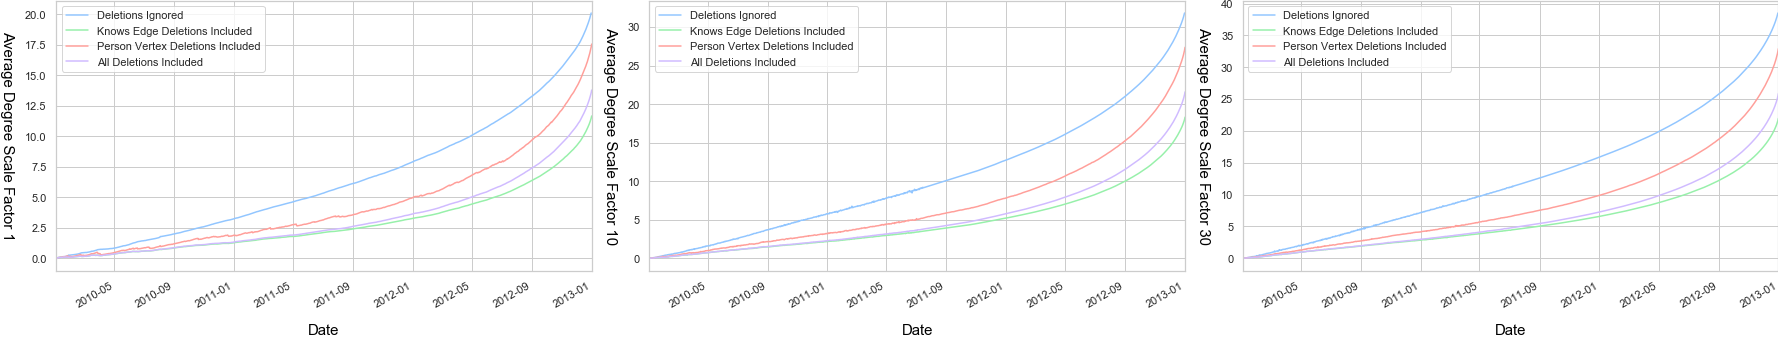
\includegraphics[width=\textwidth]{figures/degree-average-through-time-white}
%   \caption{Average $\type{know}$ degree for $\type{Person}$s in the network, measured once per day throughout the simulation period. For each scale factor, measurements were taken on four graphs built from the generated updates varying the deletions included. Experiment repeated across Scale Factors 1, 10, and 30.}
%   \label{fig:degrees}
% \end{figure*}

\subsection{Forum}
\label{sec:forum}
\label{sec:hasModerator}

A \tForum is a meeting point where people post \tMessages.
There exists three categories of \tForums:
Wall ($\eForum_\textsf{w}$),
Album ($\eForum_\textsf{a}$),
and Group ($\eForum_\textsf{g}$).
Each \tForum has a set of \tPersons connected via \tHasMember edges, a set of \tTags connected via \tHasTag edges, a single moderator connected by a \tHasModerator edge and a set of \tMessages (discussed in Section \ref{sec:message}).
For all \tForums the outgoing \tHasTag edges get their creation date and deletion date from $\varc{\eForum}$ and $\vard{\eForum}$, respectively.

\subsubsection{Groups}
Groups are public places for people that share interests, any \tPerson can create a Group $\eForum_\textsf{g}$ during their lifespan. A Group can be deleted anytime after it was created.
\begin{itemize}
    \item $\varc{\eForum}_{\mathsf{g}} \in \interval{\varc{\ePerson} + \Delta}{\min (\vard{\ePerson}, \xSE)}$
    \item $\vard{\eForum}_{\mathsf{g}} \in \interval{\varc{\eForum}_{\mathsf{g}} + \Delta}{\xNC}$
\end{itemize}

\paragraph{Group Moderator}
The initial \tHasModerator $\eHasModerator_{\mathsf{g}}$ is the Group creator. If the moderator leaves the Group, the Group will have no moderator (this is allowed in the schema of version 0.4.0+, see \autoref{fig:schema}).
\begin{itemize}
\item $\varc{\eHasModerator}_{\mathsf{g}} \in \interval{\varc{\eForum}_{\mathsf{g}} + \Delta}{\min (\vard{\eForum}_{\mathsf{g}}, \vard{\ePerson}, \xSE)}$
\item $\vard{\eHasModerator}_{\mathsf{g}} \in \interval{ \varc{\eHasModerator}_{\mathsf{g}} + \Delta}{\min (\vard{\eForum}_{\mathsf{g}}, \vard{\ePerson})}$
\end{itemize}

\paragraph{Group Membership}
Any \tPerson $\ePerson$ can become a member of a given group. The \tHasMember $\eHasMember_{\mathsf{g}}$ creation is generated from the interval in which the \tPerson and \tForum lifespans overlap. The deletion date is generated from the interval between the membership creation date (incremented by $\Delta$) and the minimum of the \tPerson and \tForum deletion dates.
\begin{itemize}
    \item $\varc{\eHasMember}_{\mathsf{g}} \in \interval{\max ( \varc{\eForum}_{\mathsf{g}}, \varc{\ePerson}) + \Delta}{\min (\vard{\eForum}, \vard{\ePerson}, \xSE)} $
    \item $\vard{\eHasMember}_{\mathsf{g}} \in \interval{\varc{\eHasMember}_{\mathsf{g}} + \Delta}{\min (\vard{\eForum}_{\mathsf{g}}, \vard{\ePerson})}$
\end{itemize}

\subsubsection{Walls}
Every \tPerson $\ePerson$, has a Wall $\eForum_\textsf{w}$ which is created when the \tPerson joins the social network. The wall is deleted when the \tPerson is deleted.
\begin{itemize}
    \item $\varc{\eForum}_{\mathsf{w}} = \varc{\ePerson} + \Delta$
    \item $\vard{\eForum}_{\mathsf{w}} = \vard{\ePerson}$
\end{itemize}

\paragraph{Wall Moderator}
Each \tPerson has a \tHasModerator $\eHasModerator_{\mathsf{w}}$ edge to their wall, which gets the creation date (incremented by $\Delta$) and deletion date from $\eForum_\textsf{w}$.
Note, only the moderator can create \tPost nodes on the wall and the connecting \tTag nodes are set based on the interest of the moderator.
\begin{itemize}
    \item $\varc{\eHasModerator}_{\mathsf{w}} = \varc{\eForum}_{\mathsf{w}} + \Delta$
    \item $\vard{\eHasModerator}_{\mathsf{w}} = \vard{\eForum}_{\mathsf{w}}$
\end{itemize}

\paragraph{Wall Membership}
For a \tPerson $p_i$, all their friends $p_j$ (\tPerson nodes connected via a \tKnows edge) become members of $\eForum_\textsf{w}$ at the time the \tKnows edge is created. Hence, a \tHasMember $\eHasMember_{\mathsf{w}}$ edge gets the creation date of \tKnows incremented by $\Delta$. The deletion date is derived from the minimum of the \tForum deletion date and \tKnows deletion date.
\begin{itemize}
    \item $\varc{\eHasMember}_{\mathsf{w}} = \varc{\eKnows_{i,j}} + \Delta$
    \item $\vard{\eHasMember}_{\mathsf{w}} = \min(\vard{\eForum}_{\mathsf{w}}, \vard{\eKnows_{i,j}})$
\end{itemize}

\subsubsection{Albums}
A \tPerson can create multiple Albums ($\eForum_\textsf{a}$) containing a set of \tPhotos{}. Albums can be created and then deleted at any point during the lifespan of the \tPerson.
\begin{itemize}
    \item $\varc{\eForum}_\textsf{a} \in \interval{\varc{\ePerson} + \Delta}{\min (\vard{\ePerson}, \xSE)}$
    \item $\vard{\eForum}_\textsf{a} \in \interval{ \varc{\eForum}_\textsf{a} + \Delta}{\vard{\ePerson}}$
\end{itemize}

\paragraph{Album Moderator}
The \tPerson is the moderator for any Album they create. Album ownership cannot change hence \tHasModerator $\eHasModerator_{\mathsf{a}}$ gets the creation date (incremented by $\Delta$) and deletion date from $\varc{\eForum}_\textsf{a}$ and $\vard{\eForum}_\textsf{a}$ respectively.
\begin{itemize}
\item $\varc{\eHasModerator}_{\mathsf{a}} = \varc{\eForum}_{\mathsf{a}} + \Delta$
\item $\vard{\eHasModerator}_{\mathsf{a}} = \vard{\eForum}_{\mathsf{a}}$
\end{itemize}

\paragraph{Album Membership}
Only friends $\ePerson_i$ of a \tPerson $\ePerson_j$ can become members of Albums created by $\ePerson_j$. The \tHasMember $\eHasMember_{\mathsf{a}}$ edge creation date is derived from the Album and $\type{knows}$ creation dates. The deletion is derived from the $\type{Forum}$ and $\type{knows}$ deletion dates.
\begin{itemize}
    \item $\varc{\eHasMember}_\textsf{a} = \max ( \varc{\eForum}_\textsf{a}, \varc{\eKnows}_{i,j} ) + \Delta $
    \item $\vard{\eHasMember}_{\mathsf{w}} = \min ( \vard{\eForum}_\textsf{a}, \vard{\eKnows}_{i,j} ) $
\end{itemize}

\subsection{Message}
\label{sec:message}

A \tMessage is an abstract entity that represents a message created by a \tPerson.
There are two \tMessage subtypes: \tPost and \tComment.
A \tPost is created in a \tForum and a \tComment represents a comment made by a \tPerson to an existing \tMessage (either a \tPost or a \tComment).
In a \tForum the set of \tMessage nodes form a \emph{tree} with a \tPost node at the root and \tComment nodes for the rest.

\subsubsection{Post}

A \tPost can be created by a \tPerson in a \tForum.
Only the moderator (\ie owner) can post on a Wall or in an Album (\tHasModerator),
whereas all members including the moderator (\tHasMember/\tHasModerator) can post in a Group.
These relationships are captured with the $\eHasMember$ variable in the formulas.
\tPosts are divided in three categories, \emph{regular posts}, \emph{photos}, and \emph{flashmob posts}.

\paragraph{Regular Posts and Photos}

Regular posts capture the standard daily activity in a Group or on a Wall.
Photos are created in Albums. (Interaction with Photos is limited to \tLikes, see details in \autoref{sec:likes}). The creation date for these is determined as follows:
$$\varc{\ePost} \in \interval{\varc{\eHasMember} + \Delta}{\min (\vard{\eHasMember}, \xSE) }$$

\paragraph{Flashmob Posts}

Flashmob posts are generated around events that attract significant interest
(such as elections) that result in a spike in activity.
These events span a $2\phi$-hour time window centered around a specific event time, flashmob event $\eFlashmobEvent$, in the middle of the window; there are $\phi$ hours each side of the specific event time.
$$
\varc{\ePost} \in \interval{\max(\varc{\eHasMember} + \Delta,\eFlashmobEvent - \phi\textrm{\,h})}{\min (\vard{\eHasMember},\eFlashmobEvent + \phi\textrm{\,h},\xSE)}
$$

The deletion dates for all categories of \tPosts are determined as:
$$\vard{\ePost} \in \interval{\varc{\ePost} + \Delta}{\vard{\eHasMember}}$$

\paragraph{containerOf edge}

Each \tPost node has an incoming $\type{containerOf}$ edge which gets the same lifespan attributes as the \tPost.

\subsubsection{Comment}

A \tComment $\eComment$ is created by \tPerson $\ePerson$ as a reply to \tMessage $\eMessage$. \tComments are only made in Walls and Groups. \tComment always occur within $\gamma$~days of their parent message following a power-law distribution with mean 6.85 hours.

\begin{itemize}
    \item $\varc{\eComment} \in \interval{\max (\varc{\eMessage}, \varc{\eHasMember}) + \Delta}{\min (\vard{\eMessage}, \vard{\eHasMember}, \varc{\eMessage} + \gamma\textrm{\,d}, \xSE)}$
    \item $\vard{\eComment} \in \interval{\varc{\eComment} + \Delta}{\min (\vard{\eMessage}, \vard{\eHasMember})}$
\end{itemize}

\paragraph{replyOf edge}

\tComments always have an outgoing \tReplyOf edge with containment semantics, \ie the target \tMessage contains the \tComment. These edges get the same lifespan as their source \tComment.

\subsubsection{likes}
\label{sec:likes}

A \tLikes edge $\eLikes$ can exist between \tPerson $\ePerson$ and \tMessage $\eMessage$. Messages can only receive likes during a $\mu$-day window after their creation at which point no more activity is generated.

\begin{itemize}
    \item $\varc{\eLikes} \in \interval{\max(\varc{\ePerson}, \varc{\eMessage}) + \Delta}{\min (\vard{\ePerson}, \vard{\eMessage}, \varc{\eMessage} + \mu\textrm{\,d}, \xSE)}$
    \item $\vard{\eLikes} \in \interval{\varc{\eLikes} + \Delta}{\min (\vard{\ePerson}, \vard{\eMessage})}$
\end{itemize}

\subsection{Complex Example}
\label{sec:complex-example}

In \autoref{fig:example-graph-complex}, a complex example graph is shown with the corresponding intervals.
Both \emph{the intervals for selecting the creation and deletion date} attributes and the selected \emph{lifespan intervals} are shown.

\begin{figure*}[htp]
  \centering
  \begin{subfigure}{\linewidth}
    \tikzstyle{vertex} = [circle, minimum width=40pt,draw,inner sep=0pt]
\tikzstyle{edge} = [thick,->,>=stealth,out=180,in=0]
\usetikzlibrary{positioning}

\centering
\begin{tikzpicture}[node distance=4cm,scale=0.85,every node/.style={transform shape}]
  % nodes
  \node (forum) [vertex,xshift=0cm,yshift=0cm,fill=Forum] {\scriptsize{$\instance{F_{1}}:\type{Forum}$}};
  \node (post) [vertex,xshift=0cm,yshift=0cm,fill=Post,right of=forum] {\scriptsize{$\instance{Post_{1}}:\type{Post}$}};
  \node (comment1) [vertex,xshift=0cm,yshift=0cm,fill=Comment,right of=post] {\scriptsize{$\instance{C_{1}}:\type{Comm}$}};
  \node (comment2) [vertex,xshift=0cm,yshift=0cm,fill=Comment,right of=comment1] {\scriptsize{$\instance{C_{2}}:\type{Comm}$}};

  \node (person1) [vertex,xshift=0cm,yshift=2cm,fill=Person,left of=forum] {\tiny{$\instance{P_{1}}:\type{Person}$}};
  \node (person2) [vertex,xshift=0cm,yshift=0cm,fill=Person,left of=forum] {\scriptsize{$\instance{P_{2}}:\type{Person}$}};
  \node (person3) [vertex,xshift=0cm,yshift=0.5cm,fill=Person,below of=forum] {\scriptsize{$\instance{P_{3}}:\type{Person}$}};

  % edges
  \draw [edge] (forum) -- node [midway,above,sloped,grey] {\scriptsize{$\instance{HMD_{1}} : \type{hasModerator}$}}
  node [midway,above,xshift=1.2cm,yshift=0.9cm,align=center,text width=2.8cm] {\scriptsize{\texttt{$\instc{HMD}{1}$: Apr 01 2010}}}
  node [midway,above,xshift=1.2cm,yshift=0.5cm,align=center,text width=2.8cm] {\scriptsize{\texttt{$\instd{HMD}{1}$: Oct 02 2012}}}
  (person1);
  \draw [edge] (forum) --
  node [midway,above] {\scriptsize{$\instance{HM_{2}} : \type{hasMember}$}}
  node [midway,below,yshift=0cm,align=center,text width=2.5cm] {\scriptsize{\texttt{$\instc{HM}{2}$: Jun 15 2010}}}
  node [midway,below,yshift=-0.4cm,align=center,text width=2.5cm] {\scriptsize{\texttt{$\instd{HM}{2}$: Jul 26 2012}}}
  (person2);

  \draw [edge] (forum) --
  node [midway,above,xshift=1.2cm,yshift=0.5cm] {\scriptsize{$\instance{HM_{3}} : \type{hasMember}$}}
  node [midway,above,xshift=1cm,yshift=0.1cm,align=right,text width=2.8cm] {\scriptsize{\texttt{$\instc{HM}{3}$: Dec 08 2010}}}
  node [midway,above,xshift=1cm,yshift=-0.3cm,align=right,text width=2.8cm] {\scriptsize{\texttt{$\instd{HM}{3}$: Feb 29 2012}}} (person3);

  \draw [edge] (forum) -- node [midway,above,grey] {\scriptsize{$\instance{CO} : \type{containerOf}$}} (post);

  \draw [edge] (post) -- node [midway,above,grey] {\scriptsize{$\instance{ROF_{1}} : \type{replyOf}$}} (comment1);
  \draw [edge] (comment1) -- node [midway,above,grey] {\scriptsize{$\instance{ROF_{2}} : \type{replyOf}$}} (comment2);
  \draw [edge] (comment1)  to [out=145,in=12]  node [near start,above,grey,sloped] {\scriptsize{$\instance{HC_{1}} : \type{hasCreator}$}} (person1);
  \draw [edge] (comment2) to [out=-135,in=-90] node [near start,above,grey,sloped] {\scriptsize{$\instance{HC_{2}} : \type{hasCreator}$}} (person2);
  \draw [edge] (post) to [out=-90,in=45] node [midway,below,grey,sloped,xshift=0.2cm] {\scriptsize{$\instance{HC_{3}} : \type{hasCreator}$}}  (person3);


  \node [below of=comment1,yshift=3cm,text width=2.5cm,align=center] {\scriptsize{\texttt{$\instc{C}{1}$: Dec 17 2010}}};
  \node [below of=comment1,yshift=2.6cm,text width=2.5cm,align=center] {\scriptsize{\texttt{$\instd{C}{1}$: Dec 18 2010}}};

  \node [above of=comment2,yshift=-2.6cm,text width=2.5cm,align=center] {\scriptsize{\texttt{$\instc{C}{2}$: Dec 18 2010}}};
  \node [above of=comment2,yshift=-3cm,text width=2.5cm,align=center] {\scriptsize{\texttt{$\instd{C}{2}$: Dec 18 2010}}};

  \node [above of=post,yshift=-2.6cm,text width=2.5cm,align=center] {\scriptsize{\texttt{$\instc{Post}{1}$: Dec 16 2010}}};
  \node [above of=post,yshift=-3cm,text width=2.5cm,align=center] {\scriptsize{\texttt{$\instd{Post}{1}$: Dec 12 2011}}};

  \node [above right=0.6 cm and -0.5cm of forum,text width=2.5cm,align=center] {\scriptsize{\texttt{$\instc{F}{1}$: Apr 01 2010}}};
  \node [above right=0.2 cm and -0.5cm of forum,text width=2.5cm,align=center] {\scriptsize{\texttt{$\instd{F}{1}$: Oct 02 2012}}};

  \node [left of=person2,xshift=2cm,yshift=0cm,text width=2.5cm,align=center] {\scriptsize{\texttt{$\instc{P}{2}$: Jan 29 2010}}};
  \node [left of=person2,xshift=2cm,yshift=-0.4cm,text width=2.5cm,align=center] {\scriptsize{\texttt{$\instd{P}{2}$: Nov 15 2012}}};

  \node [left of=person1,xshift=2cm,yshift=0cm,text width=2.5cm,align=center] {\scriptsize{\texttt{$\instc{P}{1}$: Feb 08 2010}}};
  \node [left of=person1,xshift=2cm,yshift=-0.4cm,text width=2.5cm,align=center] {\scriptsize{\texttt{$\instd{P}{1}$: Dec 23 2016}}};

  \node [right of=person3,xshift=-2cm,yshift=0cm,text width=2.5cm,align=center] {\scriptsize{\texttt{$\instc{P}{3}$: Jul 21 2010}}};
  \node [right of=person3,xshift=-2cm,yshift=-0.4cm,text width=2.5cm,align=center] {\scriptsize{\texttt{$\instd{P}{3}$: Apr 17 2012}}};

\end{tikzpicture}
\vspace{-12ex} % not the most elegant approach but you can chop off the whitespace with this

    \caption{Example graph with an instance of a \tForum containing a \tMessage tree of depth 3 and its \tPerson members. Lifespan attributes (\emph{creation} and \emph{deletion dates}) are shown for each dynamic entity. Edges in grey get their lifespan attributes as per \autoref{fig:schema} and \autoref{sec:hasModerator}.}
    \label{fig:comments-graph}
  \end{subfigure}
  %
  \begin{subfigure}{\linewidth}
    \centering
    \footnotesize
    \begin{tikzpicture}[node distance=2cm,thick,scale=0.78,every node/.style={transform shape}]
      % timeline
      \draw [thick,->,>=stealth] node [above,black] {} (-1,0/1.8) -- (13,0/1.8);
      \draw [grey,thin] (-0.5,0/1.8) node [above,black] {$\xSS$} -- (-0.5,-22/1.8);
      \draw [grey,thin] (12.5,0/1.8) node [above,black] {$\xNC$} -- (12.5,-22/1.8);
      \draw [grey,thin] (11.8,0/1.8) node [above,black] {$\xSE$} -- (11.8,-22/1.8);

      % P_1
      \draw[mark=*,mark size=2pt,mark options={color=green}] plot coordinates {(0.5,-1/1.8)} node [left] {$\instance{P_1}$}
      -- plot[mark=*,mark size=2pt,mark options={color=red}] coordinates {(12,-1/1.8)};
      \shadedBox(0.5,-1/1.8,1/1.8);

      % forum^c_{g,1}
      \draw[thin,grey,<->] plot coordinates {(0.8,-2/1.8)} node [left,black,xshift=-0.2cm] {\textcolor{grey}{$\instc{F}{1}$}} node [align=right,xshift=-3.5cm,text width=4cm] {{\textcolor{green}{$\instc{P}{1} + \Delta$}}}
      -- plot[mark=*,mark size=2pt,mark options={color=blue}] coordinates {(1,-2/1.8)}
      -- plot coordinates {(11.8,-2/1.8)} node [xshift=3.0cm,text width=4cm] {{\textcolor{red}{$\min(\instd{P}{1},\xSE)$}}};
      \shadedBox(1,-2/1.8,1/1.8);

      % forum^d_{g,1}
      \draw[thin,grey,<->] plot coordinates {(1.3,-3/1.8)} node [left,black,xshift=-0.2cm] {\textcolor{grey}{$\instd{F}{1}$}} node [align=right,xshift=-4cm,text width=4cm] {{\textcolor{green}{$\instc{F}{1} + \Delta$}}}
      -- plot[mark=*,mark size=2pt,mark options={color=blue}] coordinates {(11,-3/1.8)}
      -- plot coordinates {(12.5,-3/1.8)} node [xshift=2.3cm,text width=4cm] {{\textcolor{red}{$\xNC$}}};
      \draw [grey,thin,dashed] (1,-3/1.8) -- (1,-4/1.8);
      \draw [grey,thin,dashed] (11,-3/1.8) -- (11,-4/1.8);

      % F_{g,1}
      \draw[mark=*,mark size=2pt,mark options={color=green}] plot coordinates {(1,-4/1.8)}  node [left] {$\instance{F_{1}}$}
      -- plot[mark=*,mark size=2pt,mark options={color=red}] coordinates {(11,-4/1.8)};
      \draw[mark=*,mark size=2pt,mark options={color=green}] plot coordinates {(1,-4.5/1.8)}  node [left] {$\instance{hmem_{1}}$}
      -- plot[mark=*,mark size=2pt,mark options={color=red}] coordinates {(11,-4.5/1.8)};
      \draw [thin,dashed,grey]   (1.0,-4/1.8) -- (1,-5/1.8);

      \draw [thin,dashed,gray] (2.5,-4/1.8) -- (2.5,-9/1.8);
      \draw [thin,dashed,gray] (10.5,-4/1.8) -- (10.5,-11/1.8);
      \draw [thin,dashed,gray]   (11.0,-4/1.8) -- (11,-7/1.8);

      % P_2
      \draw[mark=*,mark size=2pt,mark options={color=green}] plot coordinates {(0.2,-5/1.8)}  node [left] {$\instance{P_2}$}
      -- plot[mark=*,mark size=2pt,mark options={color=red}] coordinates {(11.25,-5/1.8)};
      \shadedBox(1,-5/1.8,1/1.8)

      % hasMember^c_{g,2}
      \draw[thin,grey,<->] plot coordinates {(1.3,-6/1.8)} node [left,black,xshift=-0.2cm] {\textcolor{grey}{$\instc{hmem}{2}$}} node [align=right,xshift=-4cm,text width=4cm] {{\textcolor{green}{{$\max ( \instc{F}{1}, \instc{P}{2}) + \Delta$}}}}
      -- plot[mark=*,mark size=2pt,mark options={color=blue}] coordinates {(1.7,-6/1.8)}
      -- plot coordinates {(11,-6/1.8)} node [xshift=3.8cm,text width=4cm] {{\textcolor{red}{$\min(\instd{F}{1},\instd{P}{2},\xSE)$}}};
      \shadedBox(1.7,-6/1.8,1/1.8);

      % hasMember^d_{g,2}
      \draw[thin,grey,<->] plot coordinates {(2,-7/1.8)} node [left,black,xshift=-0.2cm] {\textcolor{grey}{$\instd{hmem}{2}$}} node [align=right,xshift=-4.7cm,text width=4cm] {{\textcolor{green}{$\instc{hmem}{2} + \Delta$}}}
      -- plot[mark=*,mark size=2pt,mark options={color=blue}] coordinates {(10.7,-7/1.8)}
      -- plot coordinates {(11,-7/1.8)} node [xshift=3.8cm,text width=4cm] {{\textcolor{red}{$\min(\instd{F}{1}, \instd{P}{2})$}}};
      \draw [grey,thin,dashed] (1.7,-7/1.8) -- (1.7,-8/1.8);
      \draw [grey,thin,dashed] (10.7,-7/1.8) -- (10.7,-8/1.8);

      % hmem_{g,2}
      \draw[mark=*,mark size=2pt,mark options={color=green}] plot coordinates {(1.7,-8/1.8)}  node [left] {$\instance{hmem_{2}}$}
      -- plot[mark=*,mark size=2pt,mark options={color=red}] coordinates {(10.7,-8/1.8)};

      % P_3
      \draw[mark=*,mark size=2pt,mark options={color=green}] plot coordinates {(2.5,-9/1.8)}  node [left] {$\instance{P_3}$}
      -- plot[mark=*,mark size=2pt,mark options={color=red}] coordinates {(10.5,-9/1.8)};
      \shadedBox(2.5,-9/1.8,1/1.8);

      % hasMember^c_{g,3}
      \draw[thin,grey,<->] plot coordinates {(2.8,-10/1.8)} node [left,black,xshift=-0.2cm] {\textcolor{grey}{$\instc{hmem}{3}$}}
      -- plot[mark=*,mark size=2pt,mark options={color=blue}] coordinates {(3.5,-10/1.8)} node [align=right,xshift=-6.2cm,text width=4cm] {{\textcolor{green}{{$\max ( \instc{F}{1}, \instc{P}{3}) + \Delta$}}}}
      -- plot coordinates {(10.5,-10/1.8)} node [xshift=4.3cm,text width=4cm] {{\textcolor{red}{$\min(\instd{F}{1}, \instd{P}{3}, \xSE)$}}};
      \shadedBox(3.5,-10/1.8,1/1.8);

      % hasMember^d_{g,3}
      \draw[thin,grey,<->] plot coordinates {(3.8,-11/1.8)} node [left,xshift=-0.2cm,black] {\textcolor{grey}{$\instd{hmem}{3}$}} node [align=right,xshift=-6.5cm,text width=4cm] {{\textcolor{green}{$\instc{hmem}{3} + \Delta$}}}
      -- plot[mark=*,mark size=2pt,mark options={color=blue}] coordinates {(10,-11/1.8)}
      -- plot coordinates {(10.5,-11/1.8)} node [xshift=4.3cm,text width=4cm] {{\textcolor{red}{$\min(\instd{F}{1}, \instd{P}{3})$}}};
      \draw [grey,thin,dashed] (3.5,-11/1.8) -- (3.5,-12/1.8);
      \draw [grey,thin,dashed] (10,-11/1.8) -- (10,-12/1.8);

      % hmem_{g_3}

      \draw[mark=*,mark size=2pt,mark options={color=green}] plot coordinates {(3.5,-12/1.8)}  node [left] {$\instance{hmem_{3}}$}
      -- plot[mark=*,mark size=2pt,mark options={color=red}] coordinates {(10,-12/1.8)};
      \shadedBox(3.5,-12/1.8,1/1.8);
      \draw [thin,dashed,grey] (10,-12/1.8)  -- (10,-14/1.8);

      % post^c_{g,3}
      \draw[thin,grey,<->] plot coordinates {(3.8,-13/1.8)} node [left,black,xshift=-0.2cm] {\textcolor{grey}{$\instc{Post}{1}$}} node [align=right,xshift=-6.5cm,text width=4cm] {{\textcolor{green}{{$\instc{hmem}{3} + \Delta$}}}}
      -- plot[mark=*,mark size=2pt,mark options={color=blue}] coordinates {(4,-13/1.8)}
      -- plot coordinates {(10,-13/1.8)} node [xshift=4.8cm,text width=4cm] {{\textcolor{red}{$\min (\instd{hmem}{3}, \xSE)$}}};
      \shadedBox(4,-13/1.8,1/1.8);

      % post^d_{g,3}
      \draw[thin,grey,<->] plot coordinates {(4.3,-14/1.8)} node [left,black,xshift=-0.2cm] {\textcolor{grey}{$\instd{Post}{1}$}} node [align=right,xshift=-7cm,text width=4cm] {{\textcolor{green}{$\instc{Post}{1} + \Delta$}}}
      -- plot[mark=*,mark size=2pt,mark options={color=blue}] coordinates {(9.5,-14/1.8)}
      %-- plot coordinates {(10,-14/1.8)} node [xshift=4.8cm,text width=4cm] {{\textcolor{red}{$\min (\instd{hmem}{3})$}}}; %, \xNC
      -- plot coordinates {(10,-14/1.8)} node [xshift=4.8cm,text width=4cm] {{\textcolor{red}{$\instd{hmem}{3}$}}}; %, \xNC
      \draw [grey,thin,dashed] (4,-14/1.8) -- (4,-15/1.8);
      \draw [grey,thin,dashed] (9.5,-14/1.8) -- (9.5,-15/1.8);

      % Post_{3}
      \draw[mark=*,mark size=2pt,mark options={color=green}] plot coordinates {(4,-15/1.8)}  node [left] {$\instance{Post_1}$}
      -- plot[mark=*,mark size=2pt,mark options={color=red}] coordinates {(9.5,-15/1.8)};
      \draw [thin,dashed,grey] (5.3,-15/1.8)  -- (5.3,-16/1.8);

      % comment^c_{g,1}
      \draw[thin,grey,<->] plot coordinates {(4.3,-16/1.8)} node [left,black,xshift=-0.2cm] {\textcolor{grey}{$\instc{C}{1}$}} node [align=right,xshift=-7cm,text width=4cm] {{\textcolor{green}{{$\max (\instc{Post}{1}, \instc{hmem}{1}) + \Delta$}}}}
      -- plot[mark=*,mark size=2pt,mark options={color=blue}] coordinates {(4.8,-16/1.8)}
      -- plot coordinates {(5.3,-16/1.8)} node [xshift=9.5cm,text width=4cm] {{\textcolor{red}{$\min (\instc{Post}{1} + \gamma\,\mathrm{d}, \instd{hmem}{1}, \xSE)$}}};
      \shadedBox(4,-15/1.8,1/1.8);

      % comment^d_{g,1}
      \draw[thin,grey,<->] plot coordinates {(5.1,-17/1.8)} node [left,black,xshift=-0.2cm] {\textcolor{grey}{$\instd{C}{1}$}} node [align=right,xshift=-7.8cm,text width=4cm] {{\textcolor{green}{{$\instc{Post}{1} + \Delta$}}}}
      -- plot[mark=*,mark size=2pt,mark options={color=blue}] coordinates {(7.8,-17/1.8)}
      -- plot coordinates {(9.5,-17/1.8)} node [xshift=5.3cm,text width=4cm] {{\textcolor{red}{$\min (\instd{Post}{1}, \instd{hmem}{1})$}}}; %,\xNC
      \draw [grey,thin,dashed] (4.8,-17/1.8) -- (4.8,-18/1.8);
      \draw [grey,thin,dashed] (7.8,-17/1.8) -- (7.8,-18/1.8);

      \shadedBox(4.8,-16/1.8,1/1.8);
      \draw [thin,dashed,grey] (9.5,-15/1.8)  -- (9.5,-17/1.8);

      % C_{1}
      \draw[mark=*,mark size=2pt,mark options={color=green}] plot coordinates {(4.8,-18/1.8)}  node [left] {$\instance{C_1}$}
      -- plot[mark=*,mark size=2pt,mark options={color=red}] coordinates {(7.8,-18/1.8)};

      % comment^c_{g,2}
      \draw[thin,grey,<->] plot coordinates {(5.1,-19/1.8)} node [left,black,xshift=-0.2cm] {\textcolor{grey}{$\instc{C}{2}$}} node[align=right,xshift=-7.8cm,text width=4cm] {{\textcolor{green}{{$\max (\instc{C}{1}, \instc{hmem}{2}) + \Delta$}}}}
      -- plot[mark=*,mark size=2pt,mark options={color=blue}] coordinates {(5.5,-19/1.8)}
      -- plot coordinates {(6.1,-19/1.8)}  node [xshift=8.7cm,text width=4cm] {{\textcolor{red}{$\min (\instc{C}{1} + \gamma\,\mathrm{d}, \instd{hmem}{2}, \xSE)$}}};

      \shadedBox(4.8,-18/1.8,1/1.8);
      \draw [thin,dashed,grey] (6.1,-18/1.8)  -- (6.1,-19/1.8);
      \draw [thin,dashed,grey] (7.8,-18/1.8)  -- (7.8,-20/1.8);

      % comment^d_{g,2}
      \draw[thin,grey,<->] plot coordinates {(5.8,-20/1.8)} node [left,black,xshift=-0.2cm] {\textcolor{grey}{$\instd{C}{2}$}} node [align=right,xshift=-8.5cm,text width=4cm] {{\textcolor{green}{{$\instc{C}{1} + \Delta$}}}}
      -- plot[mark=*,mark size=2pt,mark options={color=blue}] coordinates {(6.5,-20/1.8)}
      -- plot coordinates {(7.8,-20/1.8)} node [xshift=7cm,text width=4cm] {{\textcolor{red}{$\min (\instd{C}{1}, \instd{hmem}{2})$}}}; %,\xNC
      \shadedBox(5.5,-19/1.8,1/1.8);
      \draw [grey,thin,dashed] (5.5,-20/1.8) -- (5.5,-21/1.8);
      \draw [grey,thin,dashed] (6.5,-20/1.8) -- (6.5,-21/1.8);

      % C_{2}
      \draw[mark=*,mark size=2pt,mark options={color=green}] plot coordinates {(5.5,-21/1.8)}  node [left] {$\instance{C_2}$}
      -- plot[mark=*,mark size=2pt,mark options={color=red}] coordinates {(6.5,-21/1.8)};

    \end{tikzpicture}
    \caption{Illustration of the intervals in which the \emph{creation dates} \textcolor{green}{$\bullet$} and the \emph{deletion dates} \textcolor{red}{$\bullet$} of entities can be selected. Thick black lines represent entity lifespans and thin grey lines represent valid intervals that dates can be selected in; \textcolor{blue}{$\bullet$} indicates the selected times (spanning the lifespan interval of the given entity). On the thin grey lines, thicker sections represent the minimal amount of time that must pass before selecting a value. In case of creation dates, this is used to ensure that the dependant entity exists for at least $\Delta$ time. In case of deletion dates, it is used to ensure that the entity exists for at least $\Delta$ time.}
    % the \CIRCLE is from package wasysym
    \label{fig:comment-interval}
  \end{subfigure}
  %
  \caption{Example graph and time intervals for selecting lifespan attributes, \emph{creation} and \emph{deletion dates}.}
  \label{fig:example-graph-complex}
\end{figure*}


%As of version 0.4.0 Datagen produced a graph that was monotonically increasing in size over the simulation period, once a \tPerson joined the network they never left, they never deleted a post nor unliked a picture. In reality this far from the case, people regularly remove friends, delete comments and unlike pictures. Analysis of the now defunct social network iWiW~\cite{Lorincz2019} discovered across the network's lifetime 22\% of users deleted their accounts. Moreover, recent analysis of Facebook data found an average user has removed around 5\% of their cumulative friends [CITATION].

\section{Ensuring Realism}
\label{sec:ensuring-realism}

Capturing realistic deletion behaviour was broken down into two dimensions.
Firstly, each dynamic entity is assigned a probability of being explicitly deleted.
Second, if selected for explicit deletion, a deletion event date is selected using a distribution bound by the valid lifespan of that entity.
To make informed choices of deletion probabilities and deletion date distributions, where possible, real-world data was used.

\paragraph{Delete Person}

Lorincz \etal~\cite{Lorincz2019} have analyzed iWiW, a now-defunct Hungarian social network, observing that people with more connections are less likely to leave a social network.
When a \tPerson is generated they are assigned a \emph{maxKnows} value which indicates the amount of \tKnows connections they
will make across the lifetime of the network.
This information is then utilized to determine the probability a person is explicitly deleted using the distribution provided
in~\cite{Lorincz2019}, reproduced in~\autoref{fig:if-person}.
A deletion event date is then selected uniformly from the person's valid lifespan.
On average 3.5\% of \tPersons are deleted across the simulation period.

\begin{figure}[htb]
  \centering
  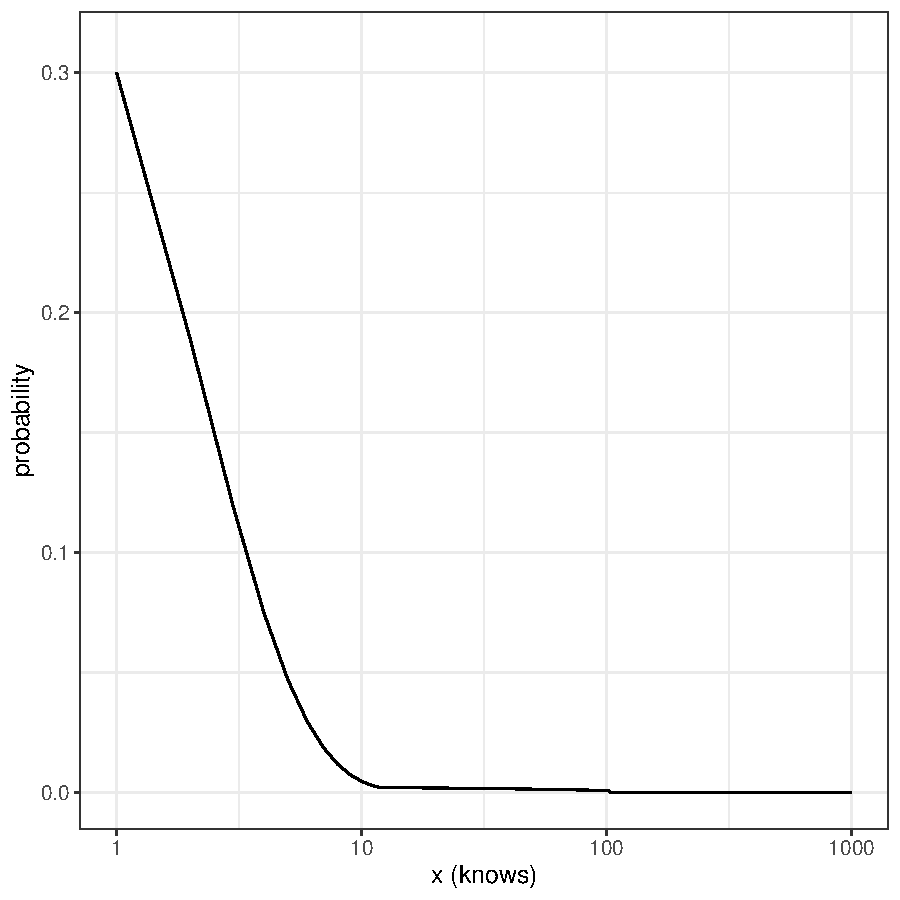
\includegraphics[scale=\yedscale]{figures/fig-if-person}
  \caption{Distribution for determining the probability a \tPerson is deleted given their number of connections.}
  \label{fig:if-person}
\end{figure}

\paragraph{Delete Knows}

Myers and Leskovec~\cite{DBLP:conf/www/MyersL14} analysed 1.2 billion tweets from 13.1 million Twitter users.
These users made 112.3 million new connections, and deleted 39.2 million connections; a 3:1 follow:unfollow ratio.
As Datagen models a generic social media platform we have chosen a different ratio of 20:1
(on average 5\% of \tKnows edges are deleted), rather than overcapture behavior that may be unique to a single site.
\cite{DBLP:conf/www/MyersL14} also finds a constant background flux of follows and unfollows interleaved with bursts in such activity.
Currently, Datagen has no follow bursts, thus, we have decided not to incorporate unfollow bursts.
They also find less similar friends have a high probability of being unfollowed; modelling this relationship is work in progress.
If a \tKnows edge is selected for explicit deletion then a deletion date is then selected uniformly from the edge's valid lifespan.

\paragraph{Delete Post/Comment and Delete Post/Comment Like}

Posts in groups and walls are produced via a uniform generator and a flashmob generator, capturing background events and bursts in
events respectively.
A comment generator is then used to produce a tree of comments on each post.
Posts in albums are referred to as photos, they are produced by a different generator and do not have flashmob events nor do they have comment trees.
Additionally, all posts and comments have a number of likes generated for it.

Almuhimedi \etal~\cite{DBLP:conf/cscw/AlmuhimediWLSA13} tracked 292K Twitter users for 1 week.
They found 2.4\% of 67.2M tweets were deleted across 4 categories: status posts, retweets, replies, and mentions of other users that
were not replies.
In order to apply these findings to Datagen and obtain the average percentage of \tMessages and \tLikes deleted across the simulation
period, tweet categories were mapped to Datagen \tMessage types.
\autoref{table:almuhimedi-mapping} gives the mapping and the percentage deleted across the simulation period within each category.

\begin{table}[H]
  \centering
  \begin{tabular}{ |c|c|c| }
    \hline
    \textbf{\cite{DBLP:conf/cscw/AlmuhimediWLSA13}} & \textbf{Datagen} & \textbf{\% Deleted} \\
    \hline\hline
    Status updates & Post/Photo & 2.7 \\
    \hline
    Non-reply mentions &  Post/Photo & 2.7 \\
    \hline
    Replies & Comment & 1.8 \\
    \hline
    Retweets & Post/Photo/Comment & 2.4 \\
    \hline
  \end{tabular}
  \centering
  \caption{Mapping of~\cite{DBLP:conf/cscw/AlmuhimediWLSA13} message types to LDBC's schema.}
  \label{table:almuhimedi-mapping}
\end{table}


Additionally, \cite{DBLP:conf/cscw/AlmuhimediWLSA13} identified not all users delete messages, with around 50\% of users doing so.
Thus, each \tPerson in the network has a 50\% chance of being marked a \emph{messageDeleter}, who subsequently, may or may not, delete post, comments, or likes.
\cite{DBLP:conf/cscw/AlmuhimediWLSA13} also identify a relationship between the depth of replies to a tweet and the chance the tweet
is deleted -- a tweet with less replies is more likely to be deleted.
We apply this relationship to the number of  \tComments in a \tPosts thread using the distribution in \autoref{fig:if-post}.
Note, this distribution has an average of 2.7\% aligning with \autoref{table:almuhimedi-mapping}.

\begin{figure}[htb]
  \centering
  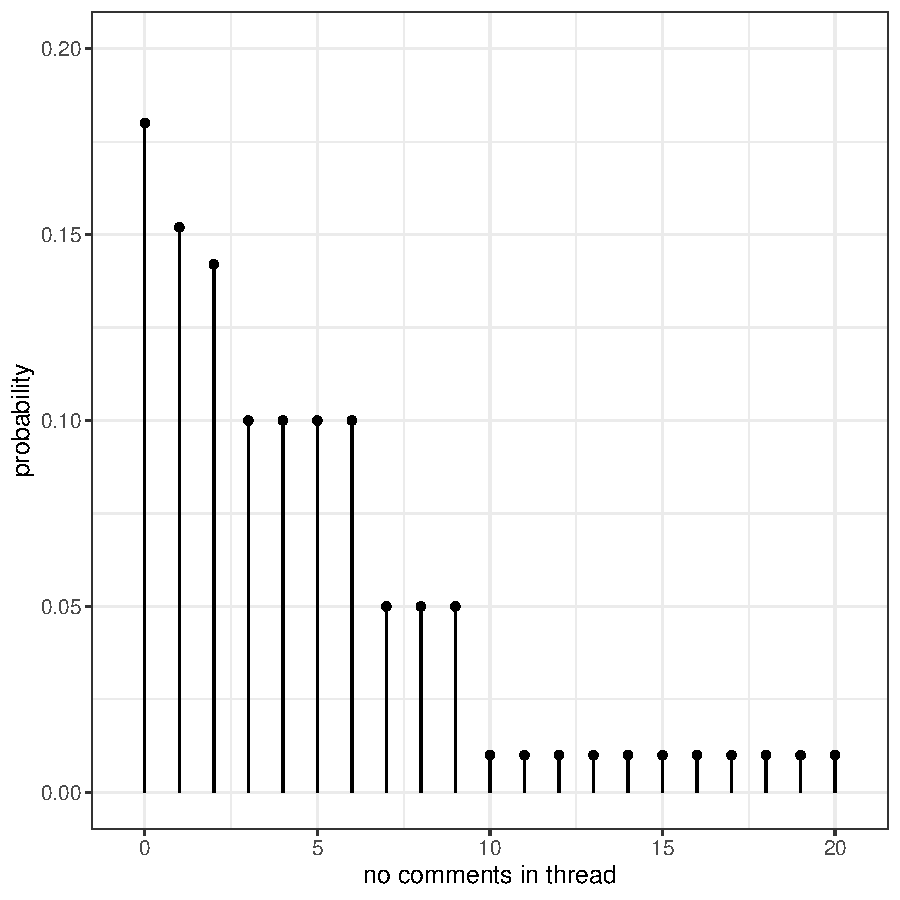
\includegraphics[scale=\yedscale]{figures/fig-if-post}
  \caption{Probability a post is deleted given the number of comments in its thread.}
  \label{fig:if-post}
\end{figure}

Almuhimedi \etal also observe a temporal relationship for when a tweet is deleted -- a tweet has a higher chance of being deleted soon
after it was created.
They found 50\% of all deleted tweets where removed within 8~minutes of creation.
We have recreated the temporal distribution in~\cite{DBLP:conf/cscw/AlmuhimediWLSA13} and use it to generate deletion dates from
the valid lifespan intervals for posts, comments, and likes that are selected for explicit deletion~\autoref{fig:when-activity}.

\begin{figure}[htb]
  \centering
  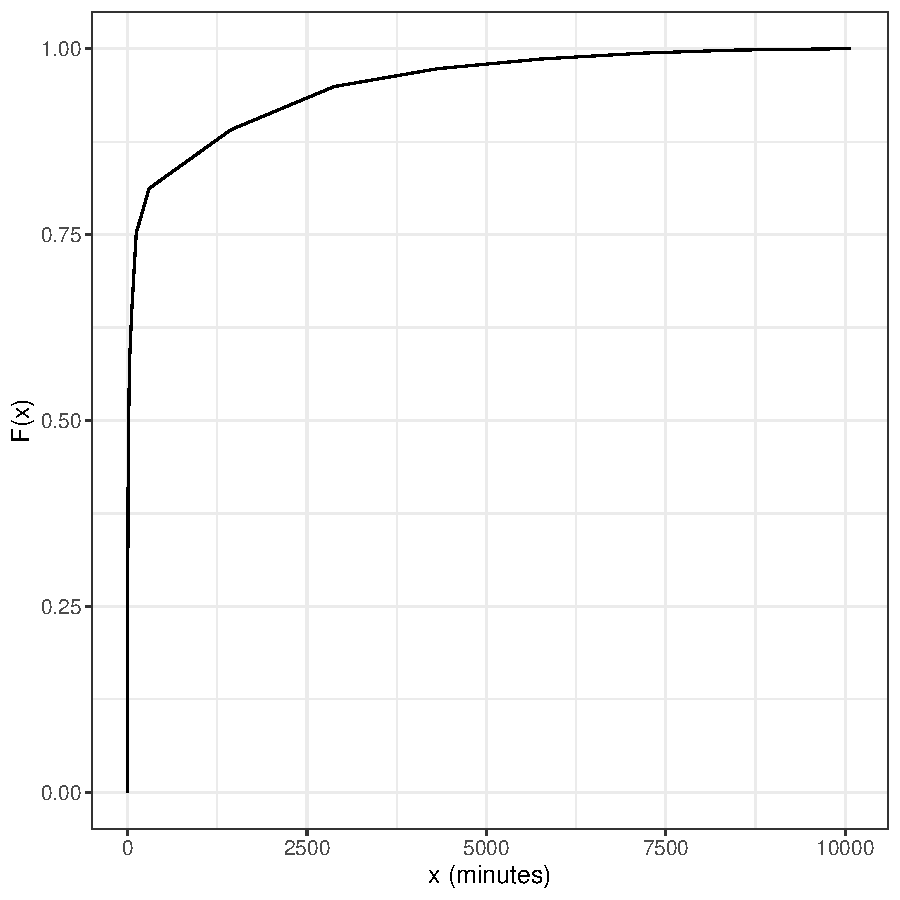
\includegraphics[scale=\yedscale]{figures/fig-when-activity}
  \caption{Cumulative probability density function of when a post, comment, or like is deleted after it is created (x = 0).}
  \label{fig:when-activity}
\end{figure}


\paragraph{Delete Forum and Delete Forum Membership}

We currently do not have empirical evidence to motivate realistic behaviour of \tForum deletion.
Forums have 3 types: walls, groups, and albums.
Groups and albums can be explicitly deleted, walls cannot.
The target proportion of groups and albums that are deleted across the simulation period is 1\%.

Additionally, we currently do not have empirical evidence to motivate realistic behaviour of \tHasMember edge deletion.
Only membership of groups can be explicitly deleted.
The target proportion of group memberships that are deleted across the simulation period is 5\%.

\section{Converting Delete Events into Delete Operations}
\label{sec:conv-delete-events}
Datagen supports 3 modes, each having different output:
\begin{itemize}
\item \textbf{Interactive}. Produces the data necessary for the Interactive workload. Includes a set of bulk load csv files and a number of update streams, which contain only insert operations.
\item \textbf{BI}. Produces the data necessary for the Business Intelligence workload. Includes a set of bulk load csv files and a number of update batches, which contain insert and delete operations.
\item \textbf{Raw}. Produces a fully dynamic graph without insert or delete operations. Includes a set of bulk load csv files (covering whole simulation period), with each dynamic entity having creation and deletion date attributes serialized. This mode is not intended for use with any LDBC workload.
\end{itemize}

When run in Interactive mode Datagen produces a graph that monotonically increases in size over the simulation period with insert-only operations, \eg once \tPerson joins the network they never leave, not delete a post nor unlike a picture.
This is mode is supported for backward compatibility with the Interactive workload.

The modes BI and raw use the dynamic graph containing creation events and deletion events.
Raw mode effectively serializes the graph to a bulk component and has a slightly different schema, with each entity having creation date and deletion date fields.
This mode was developed for testing, yet may be useful to users that require a dynamic graph data set for purposes other than benchmarking.

For the BI mode the generated data must be converted into a bulk load component and a series of update batches (containing insert and delete operations).
\autoref{fig:serialization-conds} displays the possible creation and deletion dates a dynamic entity can have with respect to the bulk load cut off, simulation end, and network collapse, which determines the target file the entity should be serialized to.
For example, if a \tPost is created after the bulk load and deleted before the simulation end this should result in a insert and a delete operation in the update batch data set.
If an entity is marked for explicit deletion then, if the conditions in \autoref{fig:serialization-conds} are satisfied then a deletion operation is serialized into the update batches.

\begin{figure}[ht]
  \centering
  \begin{subfigure}{\linewidth}
    \centering
    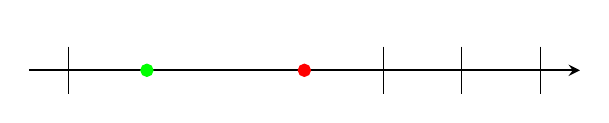
\begin{tikzpicture}[node distance=2cm,thick,every node/.style={transform shape}]
      \draw [thick,->,>=stealth] node [above,black] {} (-1,0) -- (6,0);
      \draw [thin] (-0.5,0.3) node [above,black] {$\xSS$} -- (-0.5,-0.3);
      \draw[mark=*,mark size=2pt,mark options={color=green}] plot coordinates {(0.5,0)};
      \draw[mark=*,mark size=2pt,mark options={color=red}] plot coordinates {(2.5,0)};
      \draw [thin]  (3.5,0.3) node [above,black] {$\xBL$} -- (3.5,-0.3);
      \draw [thin]  (4.5,0.3) node [above,black] {$\xSE$} -- (4.5,-0.3);
      \draw [thin]  (5.5,0.3) node [above,black] {$\xNC$} -- (5.5,-0.3);
    \end{tikzpicture}
    \caption{Dynamic entity has creation and deletion dates before the bulk load cut off. This entity is not serialized.}
    \label{fig:cond-1}
    \end{subfigure}
  %
    \begin{subfigure}{\linewidth}
    \centering
    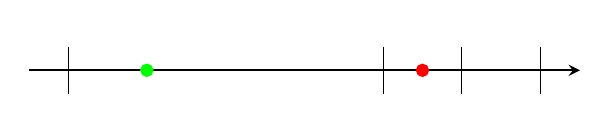
\begin{tikzpicture}[node distance=2cm,thick,every node/.style={transform shape}]
      \draw [thick,->,>=stealth] node [above,black] {} (-1,0) -- (6,0); % timeline
      \draw [thin] (-0.5,0.3) node [above,black] {$\xSS$} -- (-0.5,-0.3);
      \draw[mark=*,mark size=2pt,mark options={color=green}] plot coordinates {(0.5,0)};
      \draw [thin]  (3.5,0.3) node [above,black] {$\xBL$} -- (3.5,-0.3);
      \draw[mark=*,mark size=2pt,mark options={color=red}] plot coordinates {(4,0)};
      \draw [thin]  (4.5,0.3) node [above,black] {$\xSE$} -- (4.5,-0.3);
      \draw [thin]  (5.5,0.3) node [above,black] {$\xNC$} -- (5.5,-0.3);
    \end{tikzpicture}
        \caption{Dynamic entity has creation date before the bulk load cut off and a deletion date after the bulk load cut off, but before the simulation end. Such an entity is serialized into the bulk load component and spawns a delete operation.}
    \label{fig:cond-2}
  \end{subfigure}
  %
    \begin{subfigure}{\linewidth}
    \centering
    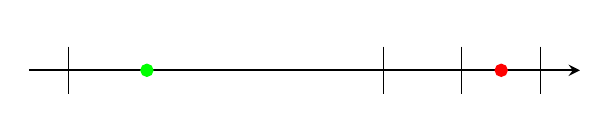
\begin{tikzpicture}[node distance=2cm,thick,every node/.style={transform shape}]
      \draw [thick,->,>=stealth] node [above,black] {} (-1,0) -- (6,0); % timeline
      \draw [thin] (-0.5,0.3) node [above,black] {$\xSS$} -- (-0.5,-0.3);
      \draw[mark=*,mark size=2pt,mark options={color=green}] plot coordinates {(0.5,0)};
      \draw [thin]  (3.5,0.3) node [above,black] {$\xBL$} -- (3.5,-0.3);
      \draw [thin]  (4.5,0.3) node [above,black] {$\xSE$} -- (4.5,-0.3);
      \draw[mark=*,mark size=2pt,mark options={color=red}] plot coordinates {(5,0)};
      \draw [thin]  (5.5,0.3) node [above,black] {$\xNC$} -- (5.5,-0.3);
    \end{tikzpicture}
        \caption{Dynamic entity has creation date before the bulk load cut off and a deletion date after the simulation end. Such an entity is in serialized only into the bulk load component.}
    \label{fig:cond-3}
  \end{subfigure}
    %
    \begin{subfigure}{\linewidth}
    \centering
    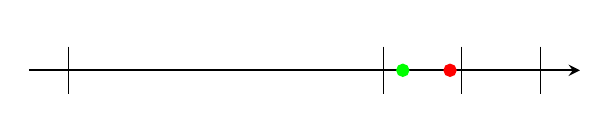
\begin{tikzpicture}[node distance=2cm,thick,every node/.style={transform shape}]
      \draw [thick,->,>=stealth] node [above,black] {} (-1,0) -- (6,0); % timeline
      \draw [thin] (-0.5,0.3) node [above,black] {$\xSS$} -- (-0.5,-0.3);
      \draw [thin]  (3.5,0.3) node [above,black] {$\xBL$} -- (3.5,-0.3);
      \draw[mark=*,mark size=2pt,mark options={color=green}] plot coordinates {(3.75,0)};
      \draw[mark=*,mark size=2pt,mark options={color=red}] plot coordinates {(4.35,0)};
      \draw [thin]  (4.5,0.3) node [above,black] {$\xSE$} -- (4.5,-0.3);
      \draw [thin]  (5.5,0.3) node [above,black] {$\xNC$} -- (5.5,-0.3);
    \end{tikzpicture}
    \caption{Dynamic entity has creation date after the bulk load cut off and a deletion date before the simulation end. Such an entity produces an insert operation and a delete operation.}
    \label{fig:cond-4}
  \end{subfigure}
    %
    \begin{subfigure}{\linewidth}
    \centering
    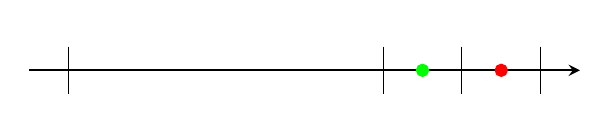
\begin{tikzpicture}[node distance=2cm,thick,every node/.style={transform shape}]
      \draw [thick,->,>=stealth] node [above,black] {} (-1,0) -- (6,0); % timeline
      \draw [thin] (-0.5,0.3) node [above,black] {$\xSS$} -- (-0.5,-0.3);
      \draw [thin]  (3.5,0.3) node [above,black] {$\xBL$} -- (3.5,-0.3);
      \draw[mark=*,mark size=2pt,mark options={color=green}] plot coordinates {(4,0)};
      \draw [thin]  (4.5,0.3) node [above,black] {$\xSE$} -- (4.5,-0.3);
      \draw[mark=*,mark size=2pt,mark options={color=red}] plot coordinates {(5,0)};
      \draw [thin]  (5.5,0.3) node [above,black] {$\xNC$} -- (5.5,-0.3);
    \end{tikzpicture}
        \caption{Dynamic entity has creation date after the bulk load cut off, but before the simulation end, and a deletion date after the simulation end. Such an entity produces only an insert operation.}
    \label{fig:cond-5}
  \end{subfigure}
  \caption{Possible dynamic entity \emph{creation} \textcolor{green}{$\bullet$} and \emph{deletion} \textcolor{red}{$\bullet$} dates with respect to simulation start, bulk load cut off, simulation end, and network collapse.}
  \label{fig:serialization-conds}
\end{figure}

